\documentclass[12pt,a4paper]{article}

% ----- Packages -----
\usepackage[utf8]{inputenc}
\usepackage{geometry}
\geometry{
  a4paper,
  top=1in,
  bottom=1in,
  left=1.25in,
  right=1in
}
\usepackage{graphicx}
\usepackage{amsmath}
\usepackage{svg} % For SVG logo support
\usepackage{hyperref}
\usepackage{setspace}
\usepackage{caption}
\usepackage{subcaption}
\usepackage{cite}
\usepackage{float}
\usepackage{titlesec}
\usepackage{enumitem}
\usepackage{tabularx}
\usepackage{longtable}
\usepackage{array}
\usepackage[none]{hyphenat} % Prevent hyphenation (words breaking across lines)
\usepackage{pgfplots}
\pgfplotsset{compat=1.18}

% ----- Formatting -----
\setlength{\parindent}{0pt}
\setlength{\parskip}{0.8em}
\onehalfspacing
\sloppy % Prevent text from spilling into margins when hyphenation is disabled

\hypersetup{
    colorlinks=true,
    linkcolor=blue,
    filecolor=magenta,      
    urlcolor=cyan,
    citecolor=blue,
}

% Rename "Contents" to "Table of Contents"
\renewcommand{\contentsname}{Table of Contents}

\begin{document}

% --- Title Page ---
\begin{titlepage}
    \centering
    
    % University Logo
    \includesvg[width=0.4\textwidth]{assets/changes/East-west-university-LogoSVG.svg}\par
    
    \vspace{1cm}
    
    {\Huge \textbf{DarkSight: A Browser Extension to Detect and Countermeasure Dark Patterns}\par}
    
    \vspace{1cm}
    
    {\LARGE \textbf{CSE400B Project Report}\par}
    
    \vspace{1.5cm}
    
    \textbf{Submitted By:}\\[0.5em]
    \large
    \textbf{Miftahul Islam Tashfin} (2022-3-60-034) \\[0.5em]
    \textbf{Nipu Basher} (2022-3-60-265) \\[0.5em]
    \textbf{Mahbubur Rahman Ovi} (2022-3-60-271) \\[0.5em]
    \textbf{Muntasir Ahmed Rifat} (2022-1-60-333) \par
    
    \vspace{1.5cm}
    
    \textbf{Supervised By:}\\[0.5em]
    \large
    \textbf{Yasin Sazid} \\
    Lecturer, Department of Computer Science and Engineering \\
    East West University\par
    
    \vfill
    
    {\large \textbf{Submission Date:} $13^{\text{th}}$ August, 2026\par}
\end{titlepage}

\newpage
\setcounter{page}{2}

% --- Abstract ---
\begin{abstract}
\noindent Dark patterns are deceptive user interface (UI) tactics engineered to subconsciously manipulate users into making decisions contrary to their best interests, such as unintended purchases or privacy concessions \cite{mathur2019, luguri}. As e-commerce platforms increasingly exploit cognitive biases and decision fatigue, pure awareness is insufficient to protect users \cite{potel}. In this project, we propose \textbf{DarkSight}, a novel, real-time browser extension that not only automatically detects dark patterns but actively mitigates them through live UI countermeasures \cite{schaefer2024}. By synthesizing landmark academic frameworks \cite{dpsentinel2024}, DarkSight employs a hybrid architecture comprising a zero-latency heuristic scanner, a local DeepSeek-R1 Large Language Model (LLM) for semantic textual analysis \cite{schaefer2023, incontext2023}, AidUI CSS structural mathematics for false hierarchy detection \cite{aidui2023}, and a Qwen2.5-VL multimodal vision model for spatial deception \cite{50shades, kocyigit2025}. Furthermore, DarkSight integrates dynamic countermeasures (Highlight, Hide, and Switch) to neutralize detected patterns in real time. Empirical evaluations demonstrate significant efficacy, achieving a 70.07\% detection accuracy on 1,818 textual instances and an 80.73\% detection accuracy on 602 visual instances. User evaluations confirm an 86\% overall satisfaction rate in restoring browsing autonomy.
\end{abstract}
\newpage

% --- Table of Contents ---
\tableofcontents
\newpage

% --- 1. Introduction ---
\section{Introduction}

\subsection{The User's Struggle and the Psychology of Manipulation}
Modern digital interfaces frequently employ psychological manipulation techniques known as "dark patterns" (or deceptive patterns) \cite{mathur2019}. These are carefully crafted UI/UX designs that exploit human cognitive biases, such as Fear Of Missing Out (FOMO), decision fatigue, and social conformity, to alter decision-making \cite{luguri}. Users subjected to these interfaces suffer from financial loss, privacy invasions, emotional stress, and a fundamental loss of digital autonomy. The ubiquitous nature of tactics like countdown timers, fake low-stock warnings, and visually suppressed "Decline" buttons highlights an urgent need for automated defensive systems \cite{bajaj2025}.

\subsection{Motivation}
While extensive academic research has identified and categorized dark patterns \cite{schaefer2023, 50shades}, user awareness alone is insufficient \cite{potel}. Users often intuitively sense that an interface is manipulative but struggle to articulate or resist the pressure while actively engaged in tasks like online shopping or account registration \cite{chen}. The psychological pressure of a ticking clock or a "selling fast" notification often overrides rational decision-making. Consequently, there is a critical need for an active, automated defense mechanism that operates in real time to shift the power dynamic back to the user \cite{schaefer2024}.

\subsection{Project Scope and Objectives}
This project introduces \textbf{DarkSight}, a lightweight Chrome extension that integrates state-of-the-art academic methodologies into a single, cohesive defensive tool \cite{dpsentinel2024}. The core objectives of DarkSight are to:
\begin{itemize}
    \item Develop a hybrid, multi-tier architecture capable of parsing the DOM, CSS properties, and rendered viewports simultaneously \cite{aidui2023, bajaj2025}.
    \item Accurately classify dark patterns using both semantic LLMs (DeepSeek-R1) \cite{schaefer2023} and spatial multimodal vision models (Qwen2.5-VL) \cite{50shades, kocyigit2025}.
    \item Dynamically inject visual countermeasures into the live DOM to neutralize manipulation before the user interacts with the deceptive element \cite{schaefer2024}.
\end{itemize}

\begin{figure}[htbp]
    \centering
    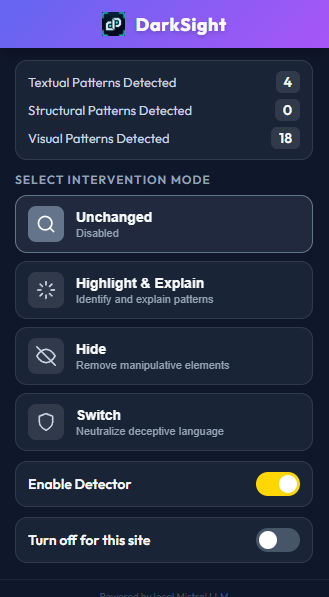
\includegraphics[width=0.3\textwidth]{assets/changes/Extension Interface.png}
    \caption{The user-facing DarkSight Chrome Extension interface, providing real-time scanning statistics and user control.}
    \label{fig:extension_ui}
\end{figure}

% --- 2. Literature Review ---
\section{Background and Literature Review}
The development of DarkSight is heavily informed by a comprehensive review of existing literature on dark pattern detection, categorization, and mitigation. We surveyed numerous foundational papers to establish our taxonomy and architecture.

\subsection{Evolution of Dark Pattern Detection}
Early detection methodologies primarily relied on static text analysis and heuristic rule-matching. Mathur et al. (2019) \cite{mathur2019} provided a foundational dataset by crawling 11K shopping websites, demonstrating that regex-based scanning is highly effective for explicit text patterns. Further studies by Vedhapriyavadhana et al. \cite{vedha} expanded on text analysis using Bidirectional Encoder Representations from Transformers (BERT) to classify shopping website deceptions. However, researchers quickly noted that text analysis alone is insufficient. Luguri and Strahilevitz \cite{luguri} demonstrated the severe impact of these patterns on user autonomy, while Chen et al. \cite{chen} unveiled similar automated tricks prevalent in mobile applications.

\subsection{The Shift to Multimodal and LLM Analysis}
As web interfaces became more dynamic, detection frameworks evolved to incorporate structural and visual information. Bajaj et al. (2025) \cite{bajaj2025} proposed comprehensive analyses utilizing structural, visual, and textual data simultaneously. The introduction of Large Language Models (LLMs) allowed for deeper semantic reasoning. Kocyigit et al. (2025) \cite{kocyigit2025} introduced "DeceptiLens," utilizing Multimodal Large Language Models (MLLMs) to support transparency in detection. Furthermore, Cuvin et al. (Stanford University) \cite{cuvin} demonstrated how dark patterns actively manipulate not just humans, but autonomous web agents, highlighting the necessity for robust, multi-layered detection.

\subsection{Active Countermeasures}
While detection is the first step, mitigation is the ultimate goal. Schäfer et al. (2024) \cite{schaefer2024} spearheaded research into "Fighting Malicious Designs" by proposing visual countermeasures against dark patterns. Similarly, Potel-Saville and Da Rocha \cite{potel} explored usable taxonomies to transition from "Dark Patterns to Fair Patterns" through active interventions. DarkSight operationalizes these theories by injecting live countermeasures (Highlight, Hide, Switch) directly into the browser DOM.

% --- 3. Examples of Deceptive UI in the Wild ---
\section{Examples of Deceptive UI in the Wild}
To contextualize the threat landscape, it is essential to examine how these manipulative designs manifest in everyday digital environments. Dark patterns are rarely accidental; they are meticulously engineered user interfaces designed to exploit cognitive biases and push users toward unintended actions. Figure \ref{fig:examples} highlights seven real-world examples of the primary manipulation tactics that the DarkSight architecture is specifically trained to detect and neutralize. These range from artificially induced scarcity on e-commerce platforms to misleading structural hierarchies in consent banners.

\begin{figure}[H]
    \centering
    \begin{subfigure}[b]{0.4\textwidth}
        \centering
        
\includegraphics[width=\textwidth]{assets/changes/forced action.png}
        \caption{Forced Action}
    \end{subfigure}
    \hfill
    \begin{subfigure}[b]{0.4\textwidth}
        \centering
        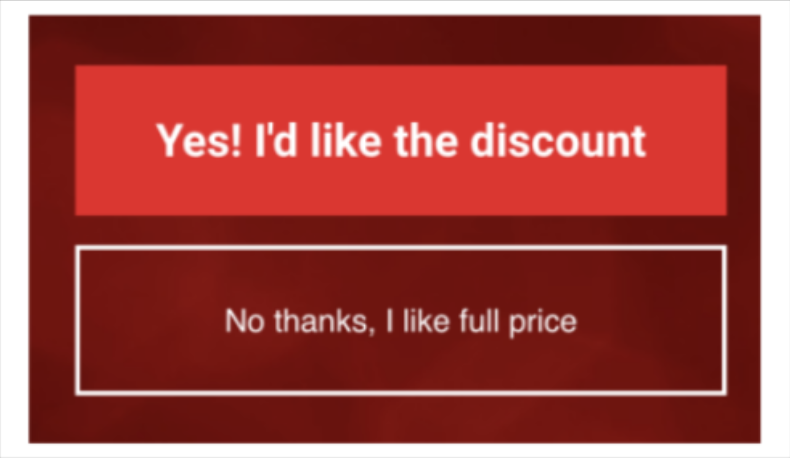
\includegraphics[width=\textwidth]{assets/changes/misdirection.png}
        \caption{Misdirection}
    \end{subfigure}
    
    \vspace{1em}
    
    \begin{subfigure}[b]{0.4\textwidth}
        \centering
        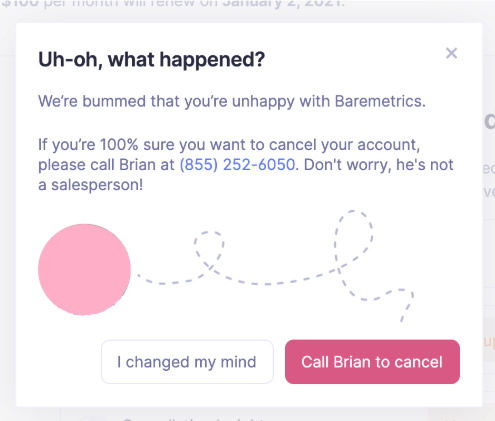
\includegraphics[width=\textwidth]{assets/changes/obstruction.png}
        \caption{Obstruction}
    \end{subfigure}
    \hfill
    \begin{subfigure}[b]{0.4\textwidth}
        \centering
        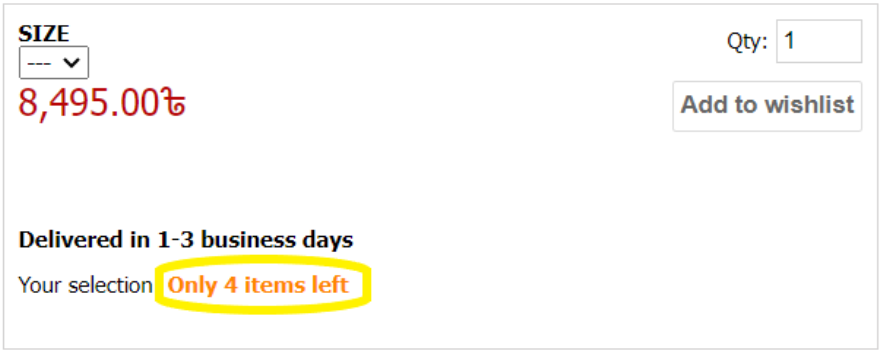
\includegraphics[width=\textwidth]{assets/changes/scarcity.png}
        \caption{Scarcity}
    \end{subfigure}
    
    \vspace{1em}
    
    \begin{subfigure}[b]{0.4\textwidth}
        \centering
        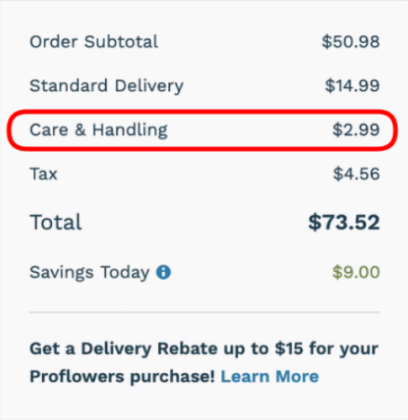
\includegraphics[width=\textwidth]{assets/changes/sneaking.png}
        \caption{Sneaking}
    \end{subfigure}
    \hfill
    \begin{subfigure}[b]{0.4\textwidth}
        \centering
        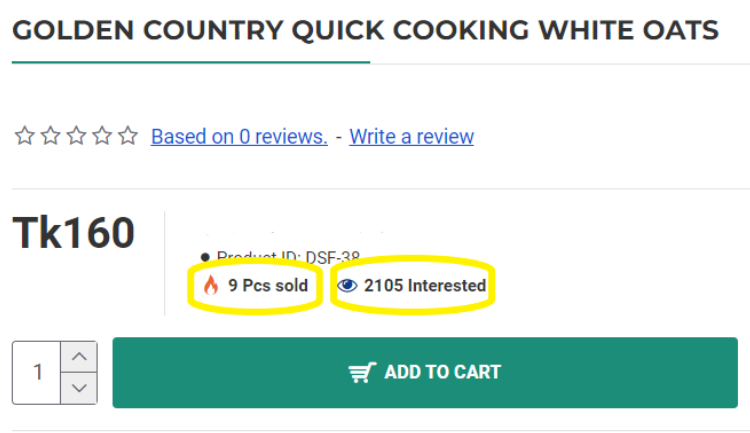
\includegraphics[width=\textwidth]{assets/changes/social proof.png}
        \caption{Social Proof}
    \end{subfigure}
    
    \vspace{1em}
    
    \begin{subfigure}[b]{0.4\textwidth}
        \centering
        
\includegraphics[width=\textwidth]{assets/changes/urgency.png}
        \caption{Urgency}
    \end{subfigure}
    
    \caption{Visual examples of the 7 core Dark Pattern categories targeted by the detection pipelines.}
    \label{fig:examples}
\end{figure}

% --- 4. Taxonomy of Deceptive Patterns ---
\section{Taxonomy of Deceptive Patterns}
To ensure rigorous classification across all detection pipelines, DarkSight synthesizes multiple academic taxonomies into structured, machine-readable engines. Rather than relying on a single source of truth, our architecture cross-references heuristic rules, structural guidelines, and visual AI frameworks to form a comprehensive defense mechanism. By clearly defining the boundaries of what constitutes manipulation versus standard marketing, we establish a robust operational framework for our algorithms.

\subsection{Textual Detection Taxonomy}
For purely textual deceptions, DarkSight utilizes a hybrid of Mathur's regex heuristics \cite{mathur2019} and Schaefer's LLM taxonomy \cite{schaefer2023}. Textual dark patterns rely heavily on manipulative language, high-pressure semantics, and deceptive phrasing to coerce users into rushed decisions. By mapping these academic definitions into our detection pipelines, DarkSight can accurately identify linguistic traps in real time. The tables below outline the core textual patterns DarkSight targets, providing a clear definition and the specific detection logic used for each.

\begin{longtable}{|p{0.2\textwidth}|p{0.4\textwidth}|p{0.3\textwidth}|}
\caption{Fast Regex Engine \cite{mathur2019}} \label{tab:regex_tax} \\
\hline
\textbf{Category} & \textbf{Explanation} & \textbf{DarkSight Detection} \\ \hline
\endfirsthead
\hline
\textbf{Category} & \textbf{Explanation} & \textbf{DarkSight Detection} \\ \hline
\endhead
\hline
\multicolumn{3}{|r|}{\textit{Continued on next page}} \\
\hline
\endfoot
\hline
\endlastfoot
Urgency & Pressuring the user to buy fast using time countdowns. & Matches "offer expires", "limited time". \\ \hline
Scarcity & Claiming inventory is almost gone to trigger FOMO. & Matches "only 2 left", "selling fast". \\ \hline
Social Proof & Showing other shoppers' actions to make the item look popular. & Matches "viewing right now", "bought in 24h". \\ \hline
Fake Discount & Misleading crossed-out price badges or exaggerated savings. & Matches "99\% OFF", "Flat 50\% discount". \\ \hline
\end{longtable}

\vspace{1em}
\noindent When regex is insufficient, the text is routed to the DeepSeek-R1 LLM using Schaefer's 8-category taxonomy \cite{schaefer2023, incontext2023}.
\vspace{1em}

\begin{longtable}{|p{0.2\textwidth}|p{0.4\textwidth}|p{0.3\textwidth}|}
\caption{Text LLM Taxonomy \cite{schaefer2023}} \label{tab:llm_tax} \\
\hline
\textbf{Category} & \textbf{Explanation} & \textbf{DarkSight Detection} \\ \hline
\endfirsthead
\hline
\textbf{Category} & \textbf{Explanation} & \textbf{DarkSight Detection} \\ \hline
\endhead
\hline
\multicolumn{3}{|r|}{\textit{Continued on next page}} \\
\hline
\endfoot
\hline
\endlastfoot
Misdirection & Distracting the user or using emotional guilt. & Flags confirmshaming text. \\ \hline
Urgency & Manipulative time pressure beyond simple regex. & Evaluates paragraph context for pressure. \\ \hline
Scarcity & Inventory pressure embedded in descriptions. & Flags subtle artificial scarcity claims. \\ \hline
Social Proof & Testimonials designed to force quick decisions. & Detects unverified popularity claims. \\ \hline
Obstruction & Making cancellation unnecessarily hard. & Flags complex steps to cancel. \\ \hline
Forced Action & Forcing users to accept marketing consent. & Flags mandatory agreement checkboxes. \\ \hline
Sneaking & Hiding hidden fees or care costs. & Detects stealth charges in terms. \\ \hline
Fake Discount & Suspicious slash pricing or unrealistic bait. & Flags absurd discount claims. \\ \hline
\end{longtable}

\subsection{Structural and Visual Taxonomy}
For UI layouts that manipulate visual hierarchy, DarkSight relies on the AidUI engine \cite{aidui2023} and the "50 Shades of Deceptive Patterns" 21-category visual taxonomy \cite{50shades}.

\begin{longtable}{|p{0.2\textwidth}|p{0.4\textwidth}|p{0.3\textwidth}|}
\caption{Structural Visual Analysis Engine \cite{aidui2023}} \label{tab:aidui_tax} \\
\hline
\textbf{Category} & \textbf{Explanation} & \textbf{DarkSight Detection} \\ \hline
\endfirsthead
\hline
\textbf{Category} & \textbf{Explanation} & \textbf{DarkSight Detection} \\ \hline
\endhead
\hline
\multicolumn{3}{|r|}{\textit{Continued on next page}} \\
\hline
\endfoot
\hline
\endlastfoot
False Hierarchy & Making the desired option giant and brightly colored, while making the alternative tiny or low-contrast. & Calculates button surface area and color contrast ratio. Flags if discrepancy $\ge$ 1. \\ \hline
\end{longtable}

\vspace{1em}
\noindent For completely graphical manipulation, the Qwen2.5-VL Multimodal model evaluates full viewport screenshots against 21 distinct visual categories \cite{50shades, dpsentinel2024}.
\vspace{1em}

\begin{longtable}{|p{0.25\textwidth}|p{0.35\textwidth}|p{0.3\textwidth}|}
\caption{21-Category Visual Taxonomy \cite{50shades}} \label{tab:vision_tax} \\
\hline
\textbf{Category} & \textbf{Explanation} & \textbf{DarkSight Detection} \\ \hline
\endfirsthead
\hline
\textbf{Category} & \textbf{Explanation} & \textbf{DarkSight Detection} \\ \hline
\endhead
\hline
\multicolumn{3}{|r|}{\textit{Continued on next page}} \\
\hline
\endfoot
\hline
\endlastfoot
False Hierarchy & Primary button dominates the screen over decline options. & Visual layout comparison of prominence. \\ \hline
Disguised Ads & Advertisements stylized to look like site menus. & Classification of ads mimicking native UI. \\ \hline
Gamification & Fake spin-the-wheel popups. & Detects interactive game popups. \\ \hline
Price Comparison Prevention & Layouts hiding unit prices to block comparison. & Detects missing comparative badges. \\ \hline
Hidden Costs & Mandatory fees revealed visually at payment. & Identifies checkout surprise additions. \\ \hline
Sneak into Basket & Extra products pre-added into the cart visually. & Flags pre-populated cart items. \\ \hline
Roach Motel & Visual design making sign-up prominent but cancellation hidden. & Identifies asymmetric user journey. \\ \hline
Confirmshaming & Decline buttons styled with guilt-inducing cues. & Flags visual buttons with guilt text. \\ \hline
Trick Questions & Confusing visual toggle switches. & Detects ambiguous slider toggles. \\ \hline
Nagging & Repetitive intrusive popups. & Identifies modal overlays obstructing reading. \\ \hline
Hard to Cancel & Deep nested menus for account cancellation. & Analyzes visual flow of settings. \\ \hline
Pre-selected Options & Checkboxes pre-filled for newsletters. & Detects checked visual box states. \\ \hline
Continuous Scroll & Endless page loading. & Identifies infinite feed UI layouts. \\ \hline
Visual Interference & Hiding unsubscribe links in tiny grey text. & Identifies low-visibility link placement. \\ \hline
Artificial Scarcity & Fake visual badges claiming limited stock. & Identifies warning icon badges. \\ \hline
Artificial Urgency & Fake graphic countdown timer widgets. & Identifies animated timer graphics. \\ \hline
Social Proof Popups & Floating toast notifications. & Detects bottom-corner purchase boxes. \\ \hline
Forced Registration & Full-screen modal wall blocking content. & Identifies backdrop blur overlays. \\ \hline
Hidden Subscriptions & Recurring billing details hidden in fine print. & Detects fine-print disclosures. \\ \hline
Defaulting & Setting privacy-invasive choices as default. & Flags pre-selected privacy options. \\ \hline
Deceptive Timers & Timers that reset visually on page refresh. & Identifies static timer widgets. \\ \hline
\end{longtable}

% --- 5. System Architecture ---
\section{DarkSight Architecture: The Sentinel Hybrid Model}
To balance computational cost with high accuracy, DarkSight orchestrates its detection modules through a tiered cascade framework \cite{dpsentinel2024}.

\begin{figure}[htbp]
    \centering
    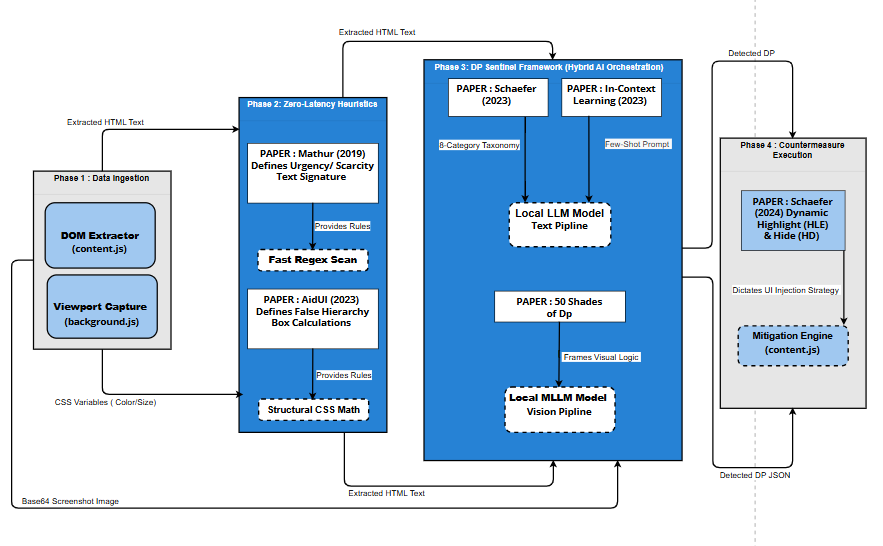
\includegraphics[width=\textwidth]{assets/changes/darksight architechture diagram.png}
    \caption{The complete DarkSight Master Architecture detailing the multi-tiered detection and mitigation pipelines.}
    \label{fig:full_arch}
\end{figure}

\subsection{Phase 1: Data Ingestion}
Data ingestion is the critical first step. DarkSight employs two distinct extraction methods simultaneously. First, the DOM Extractor traverses the page's HTML structure, isolating visible leaf-node text and extracting the calculated CSS variables (color, size) of interactive elements. Concurrently, the Viewport Capture engine encodes a high-resolution, Base64 screenshot of the user's active screen.

\begin{figure}[htbp]
    \centering
    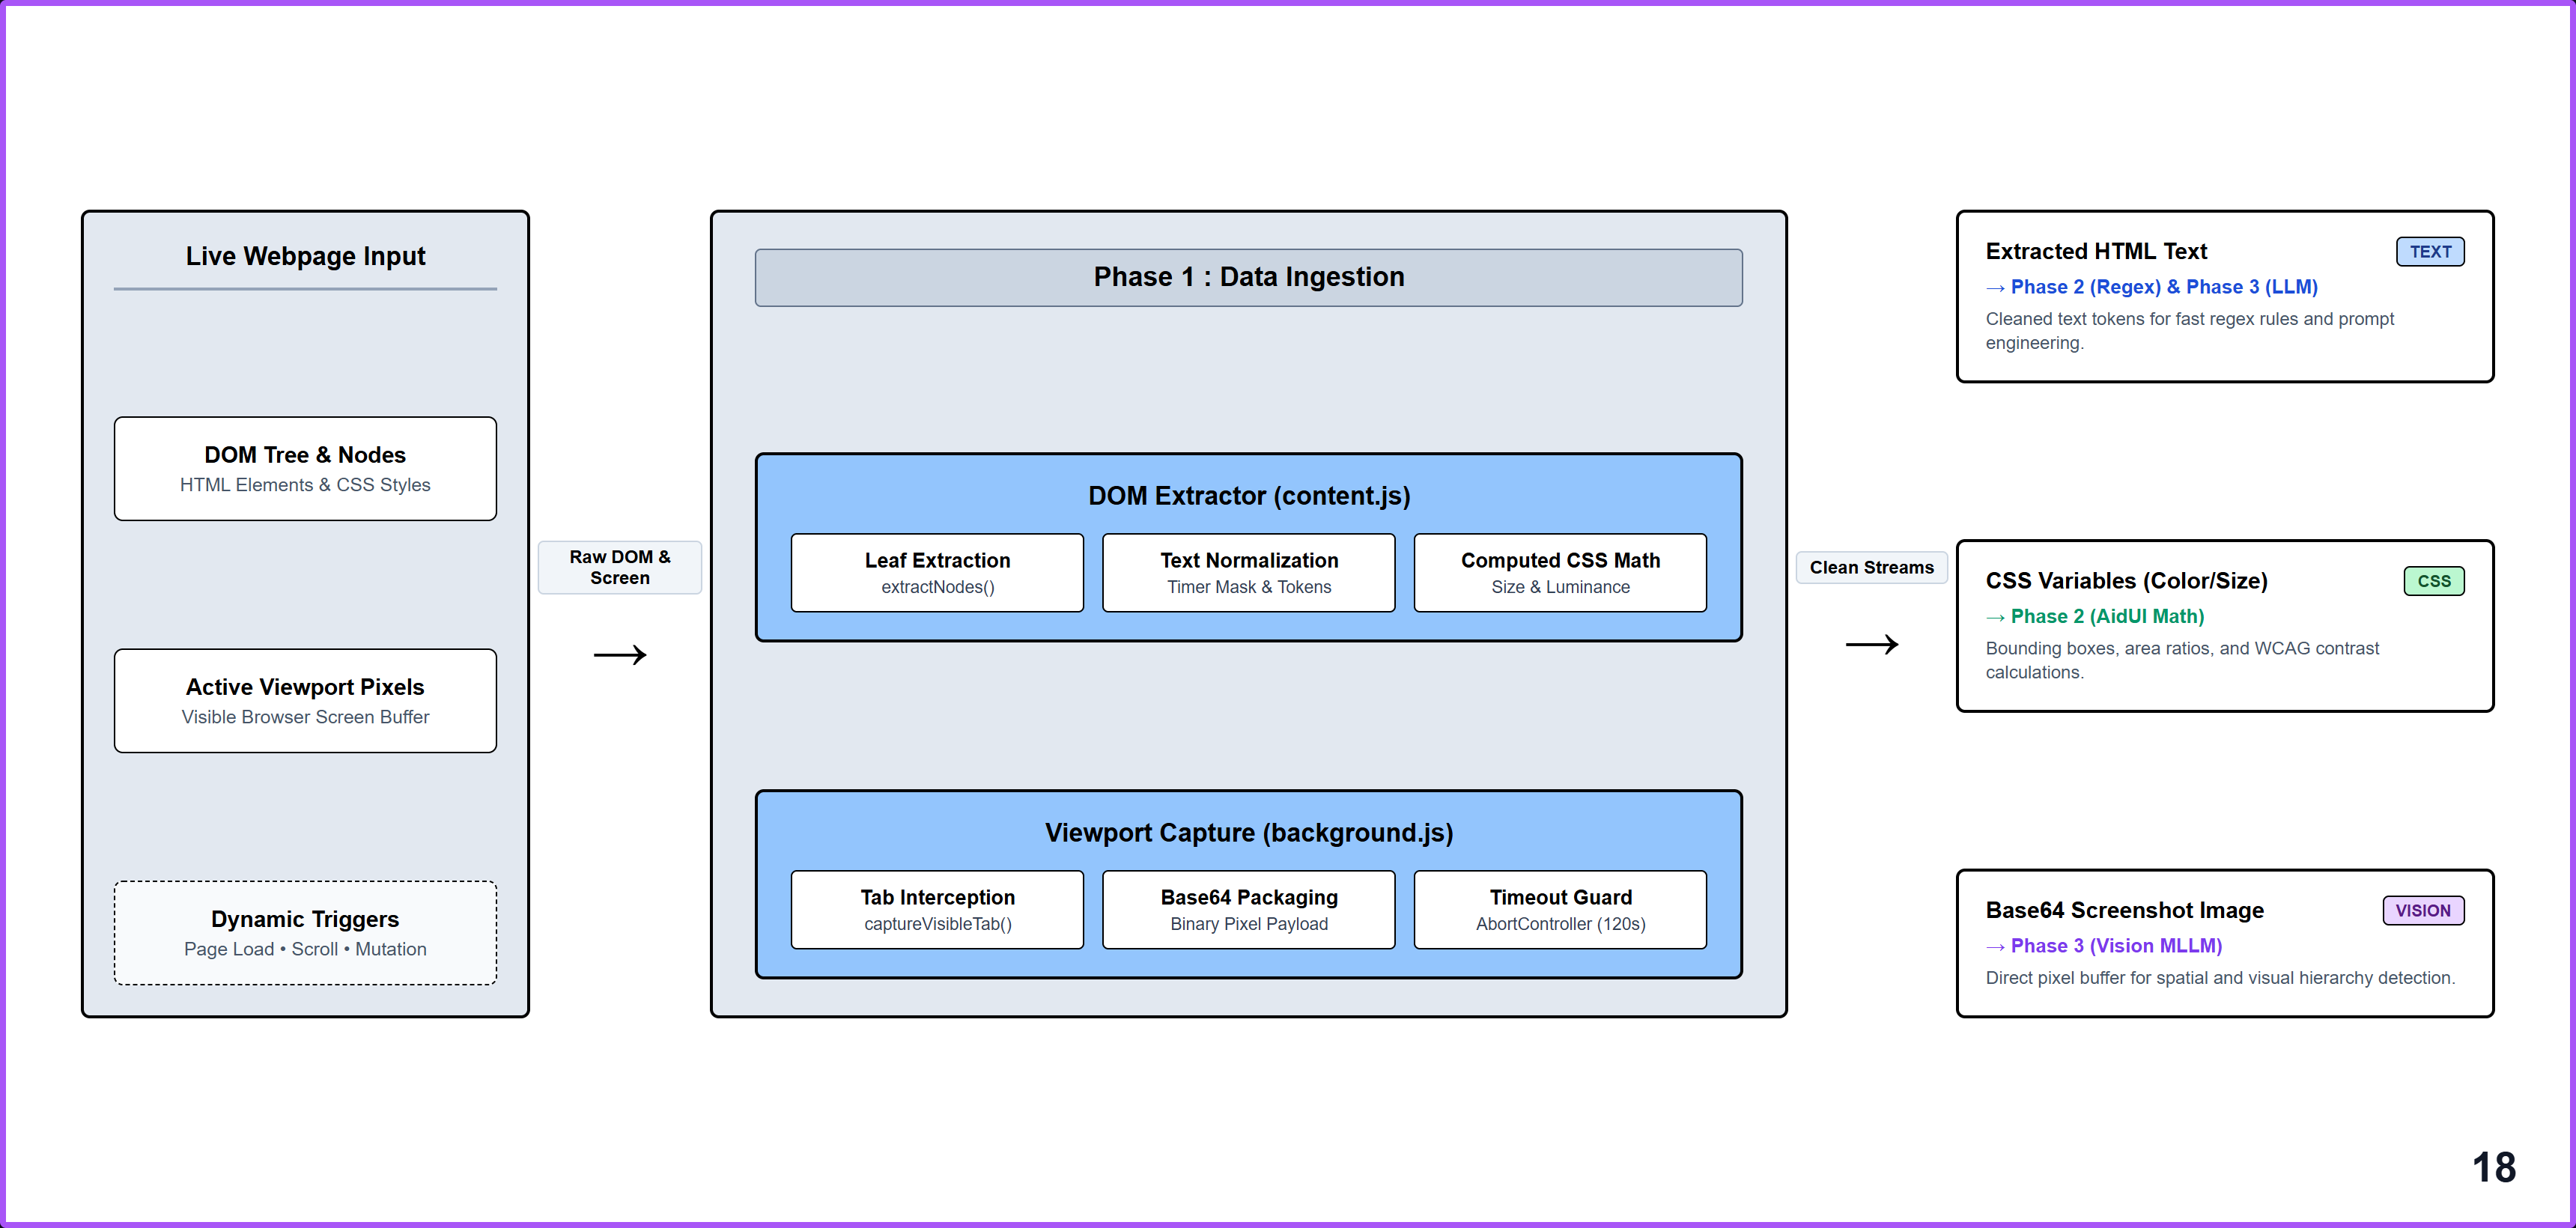
\includegraphics[width=0.8\textwidth]{assets/Phase1_Diagram_Card_Only.png}
    \caption{Phase 1: Data Ingestion separating DOM extraction and Viewport capture.}
    \label{fig:phase1}
\end{figure}

\subsection{Phase 2: Textual Detection Pipeline}
The textual pipeline evaluates semantic deception. Cleaned HTML text is first passed through a zero-latency Regex Engine \cite{mathur2019}. If the text yields a high-confidence match for explicit Urgency or Scarcity, it is instantly flagged. If the text is ambiguous, it is passed to the local DeepSeek-R1 (1.5B parameter) model \cite{schaefer2023}. Utilizing Chain-of-Thought reasoning and our taxonomy-infused prompt, the LLM determines the underlying manipulative intent before returning a confirmed dark pattern flag.

\begin{figure}[htbp]
    \centering
    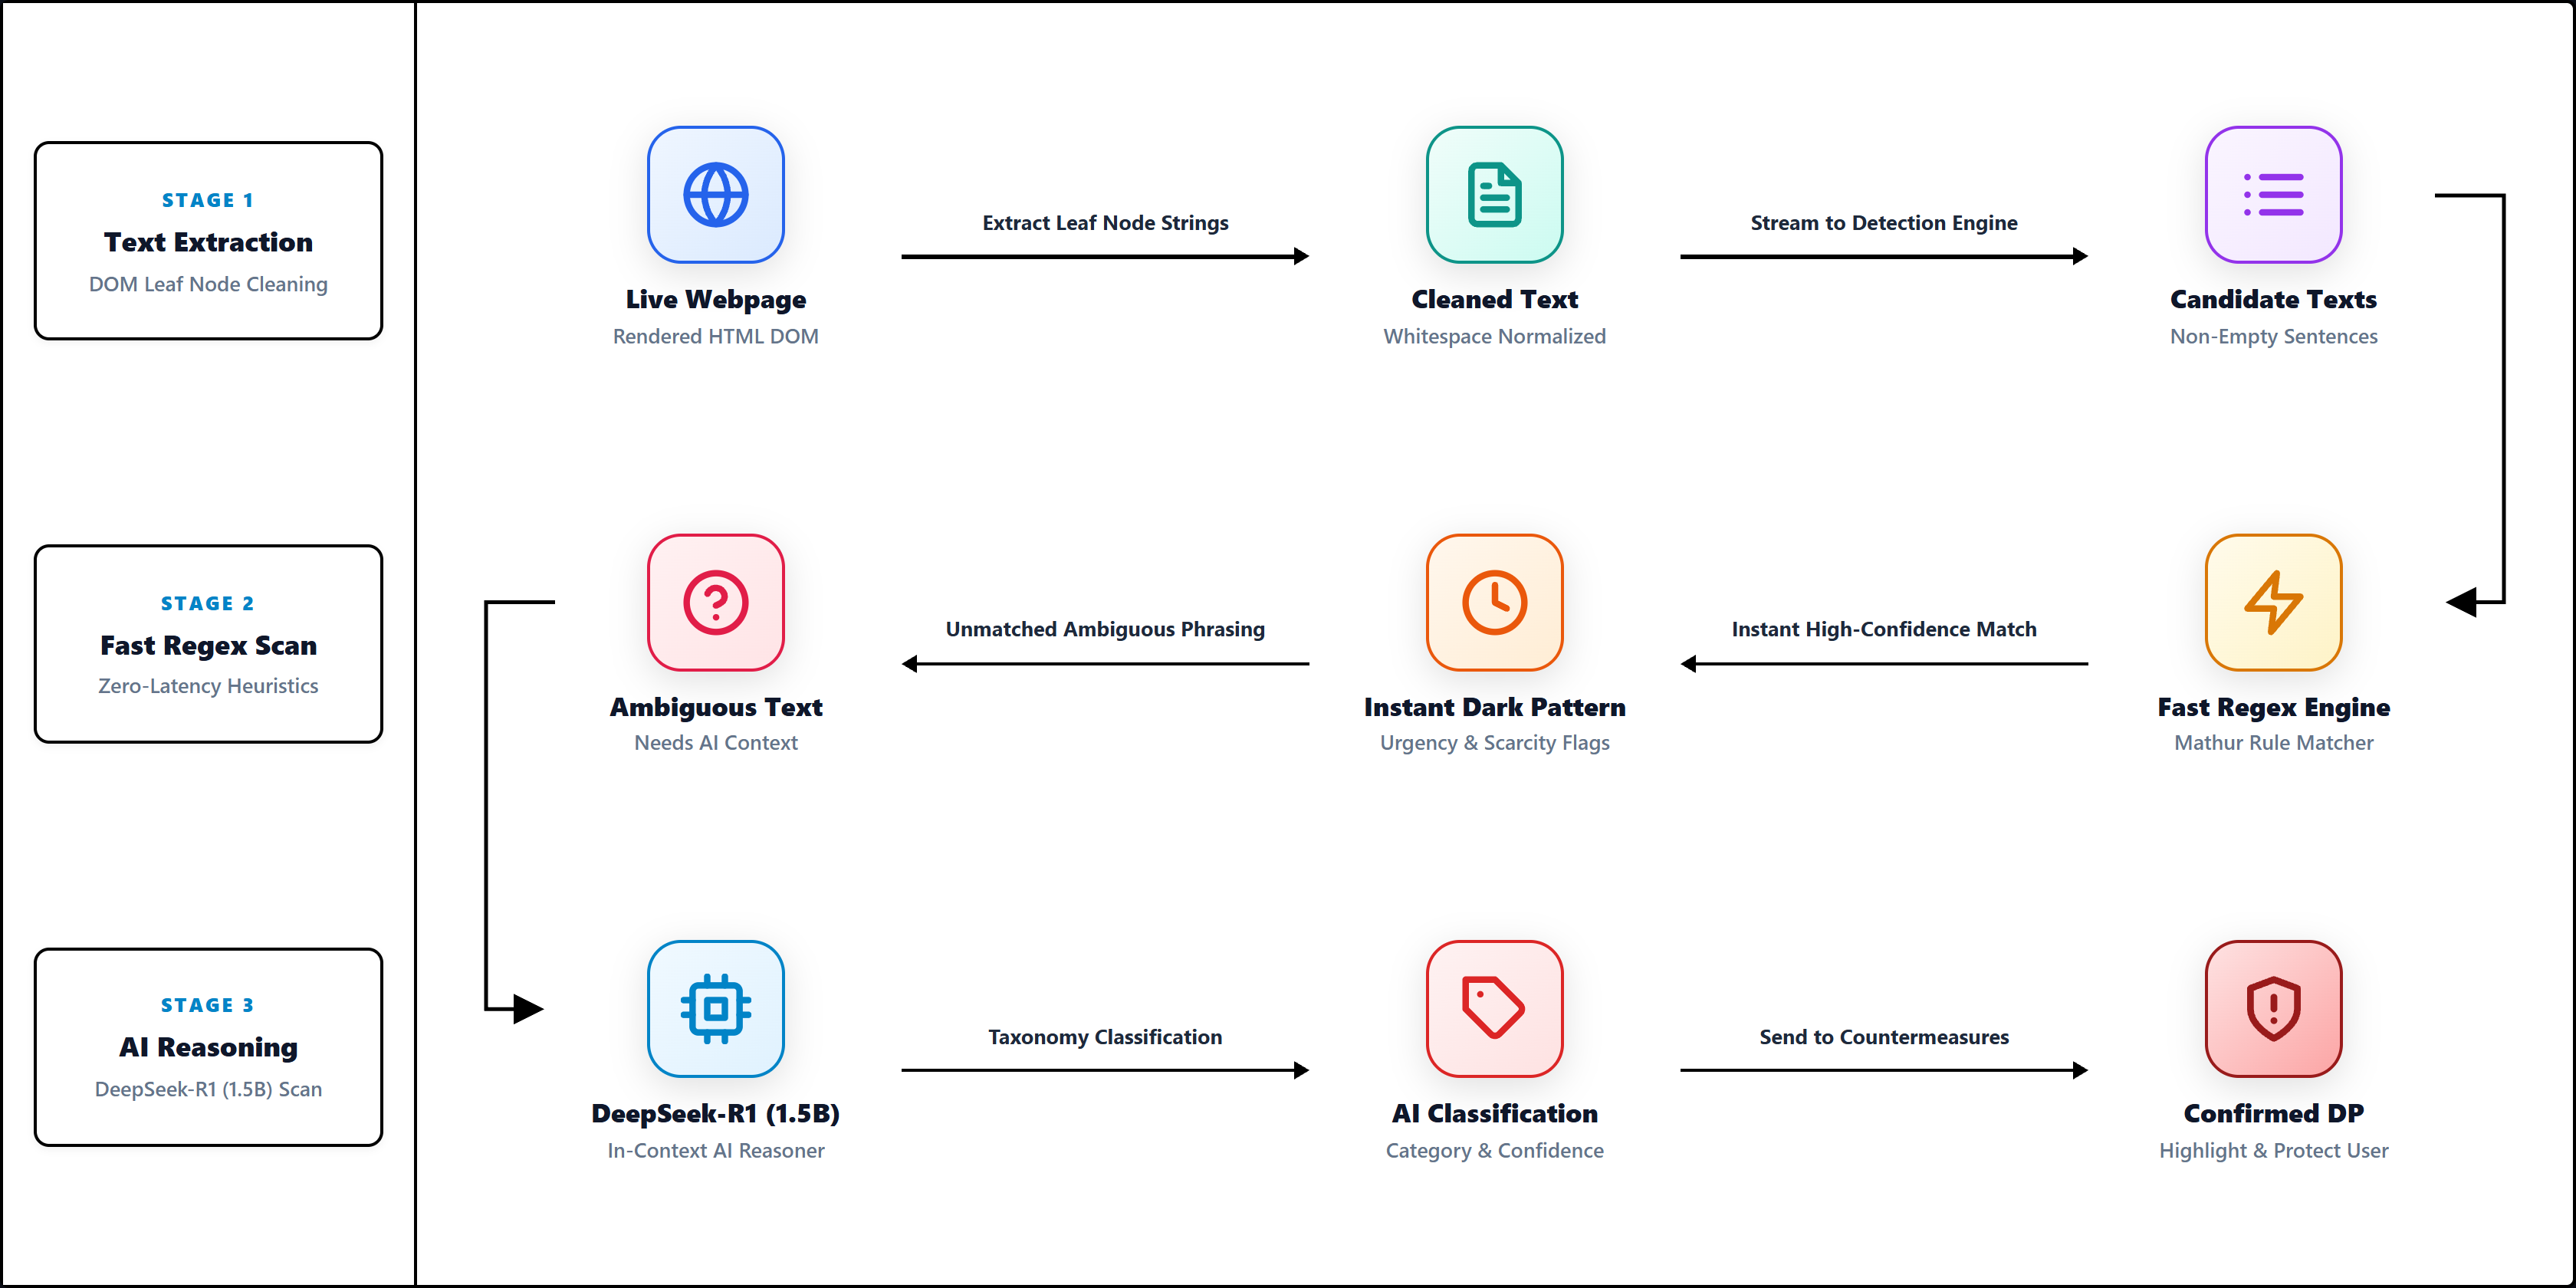
\includegraphics[width=\textwidth]{assets/Textual_Detection_Pipeline_Diagram.png}
    \caption{The Textual Detection Pipeline leveraging fast regex heuristics and local LLM reasoning.}
    \label{fig:textual_pipe}
\end{figure}

\subsection{Phase 3: Structural Detection Pipeline}
To combat UI layouts that attempt to hide choices, the Structural Detection Pipeline applies the AidUI methodology \cite{aidui2023}. It ingests adjacent interactive elements and calculates the area and color contrast asymmetry ratios. If the gap exceeds the calculated visual interference threshold, the interface is flagged for False Hierarchy or Misdirection.

\begin{figure}[htbp]
    \centering
    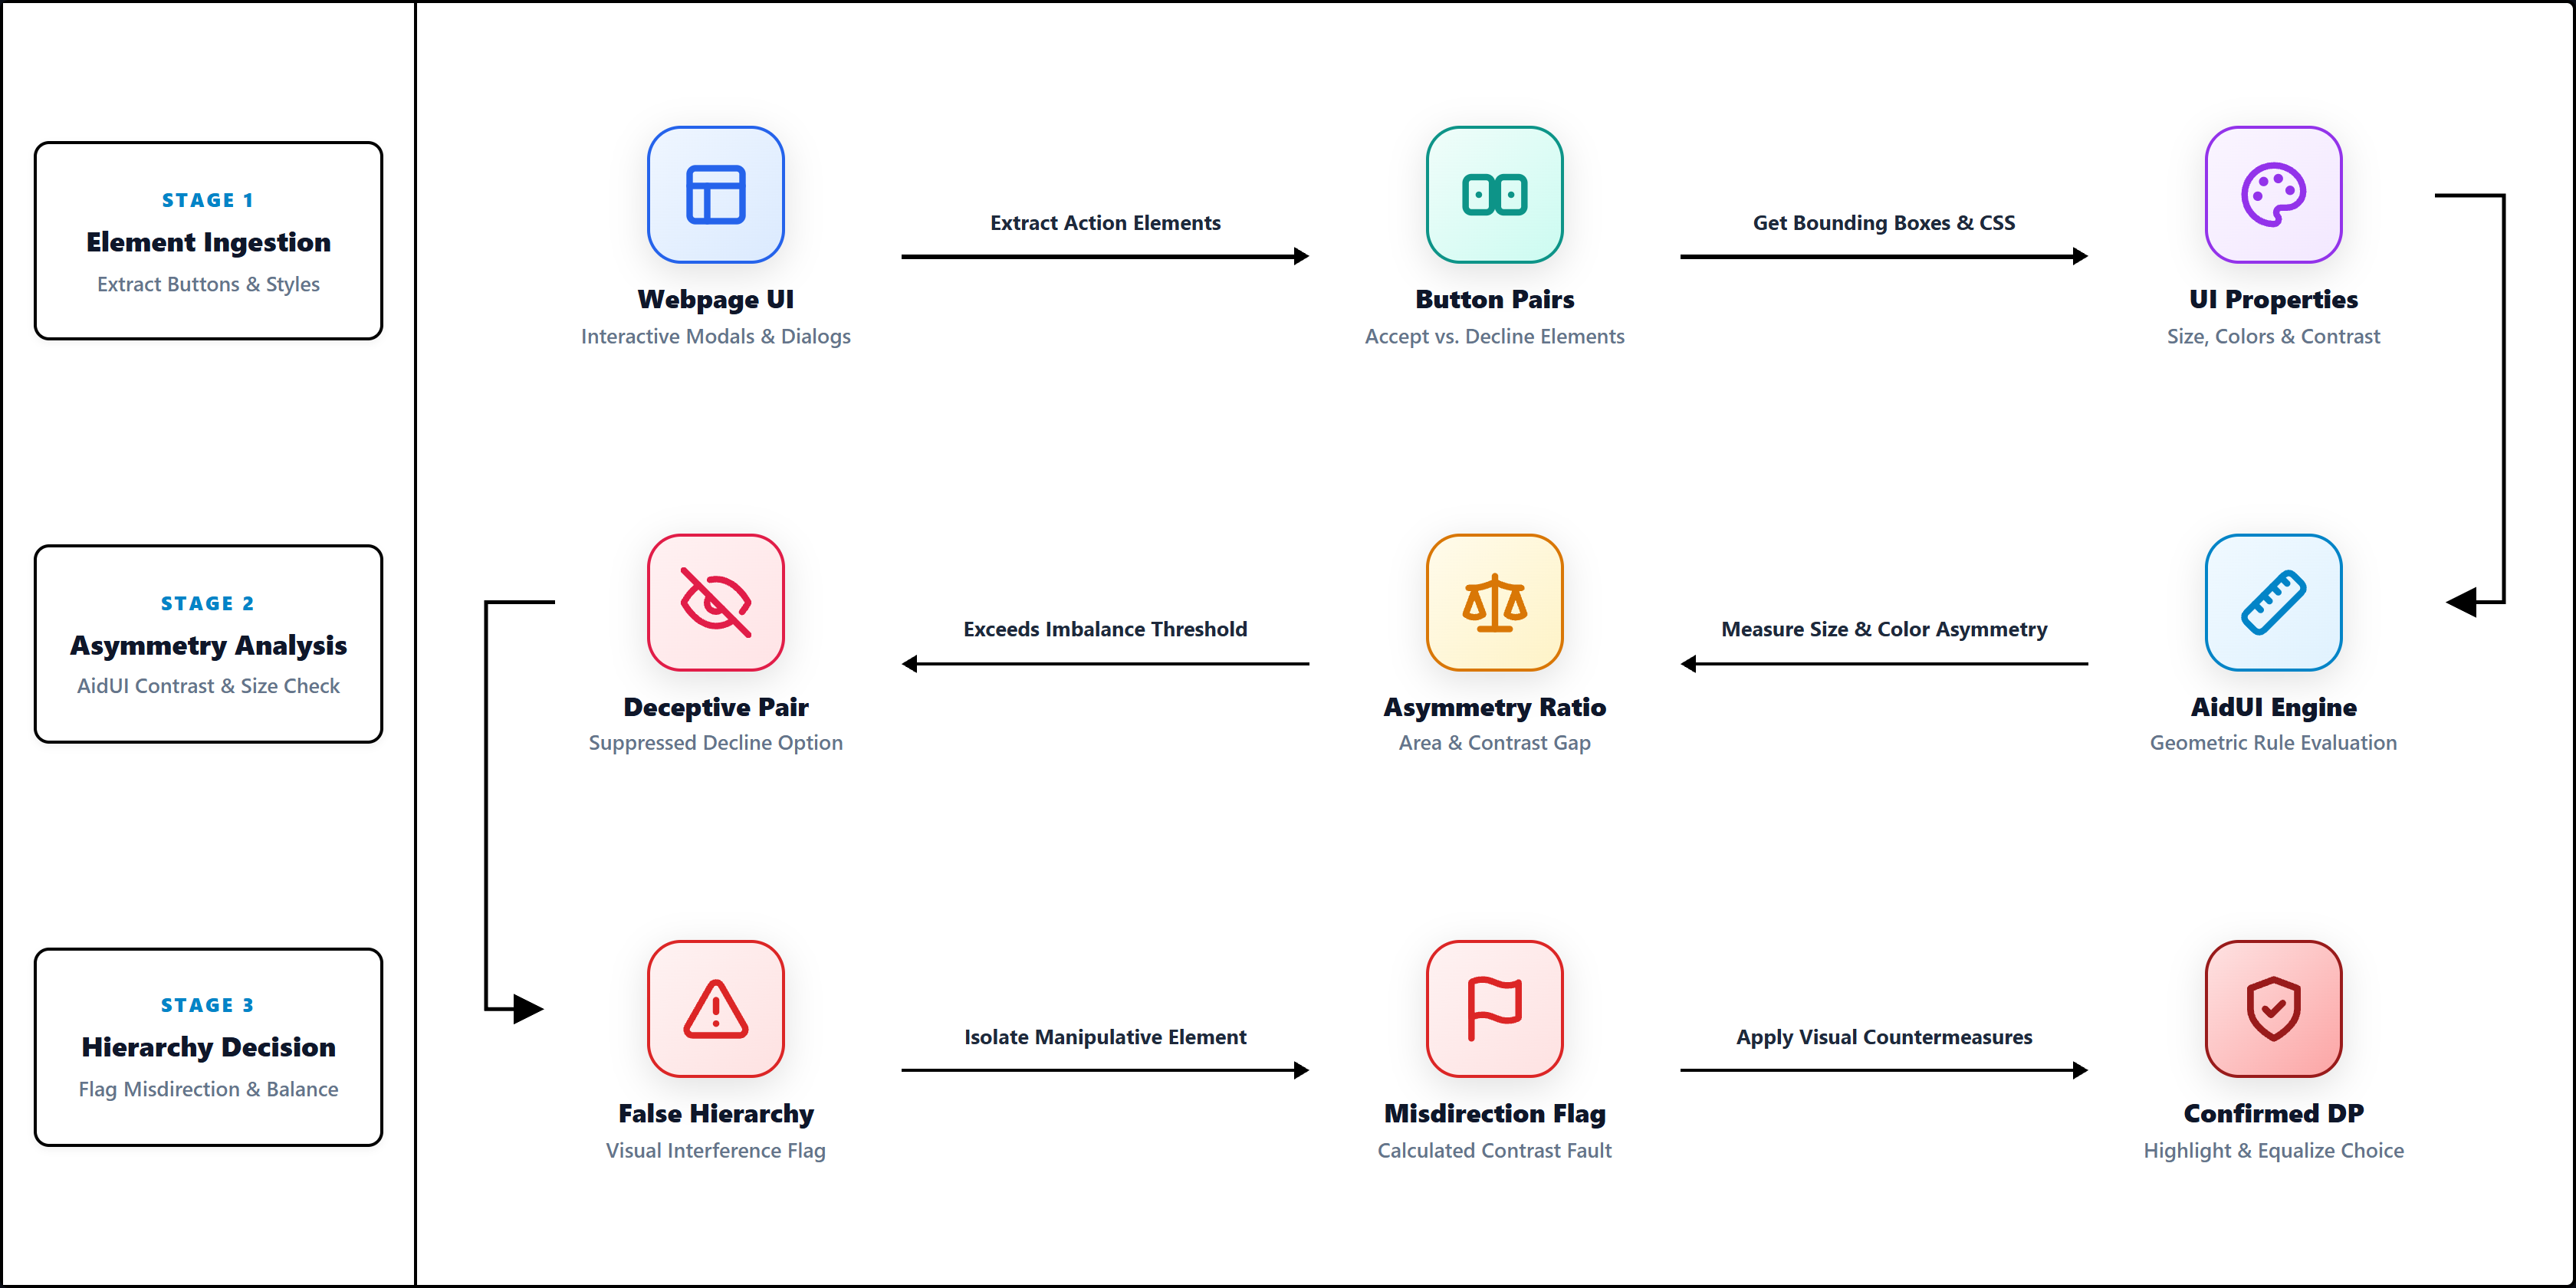
\includegraphics[width=\textwidth]{assets/Structural_Detection_Pipeline_Diagram.png}
    \caption{The Structural Detection Pipeline mathematically verifying UI symmetry.}
    \label{fig:structural_pipe}
\end{figure}

\subsection{Phase 4: Visual Detection Pipeline}
For complex deceptions that evade the DOM, the captured page snapshot is streamed to the Qwen2.5-VL multimodal vision model \cite{kocyigit2025}. Grounded by the 21-category taxonomy \cite{50shades}, the model performs spatial reasoning to identify manipulative visual elements, returning bounding box coordinates that allow DarkSight to map the deception precisely back to the user's screen resolution.

\begin{figure}[htbp]
    \centering
    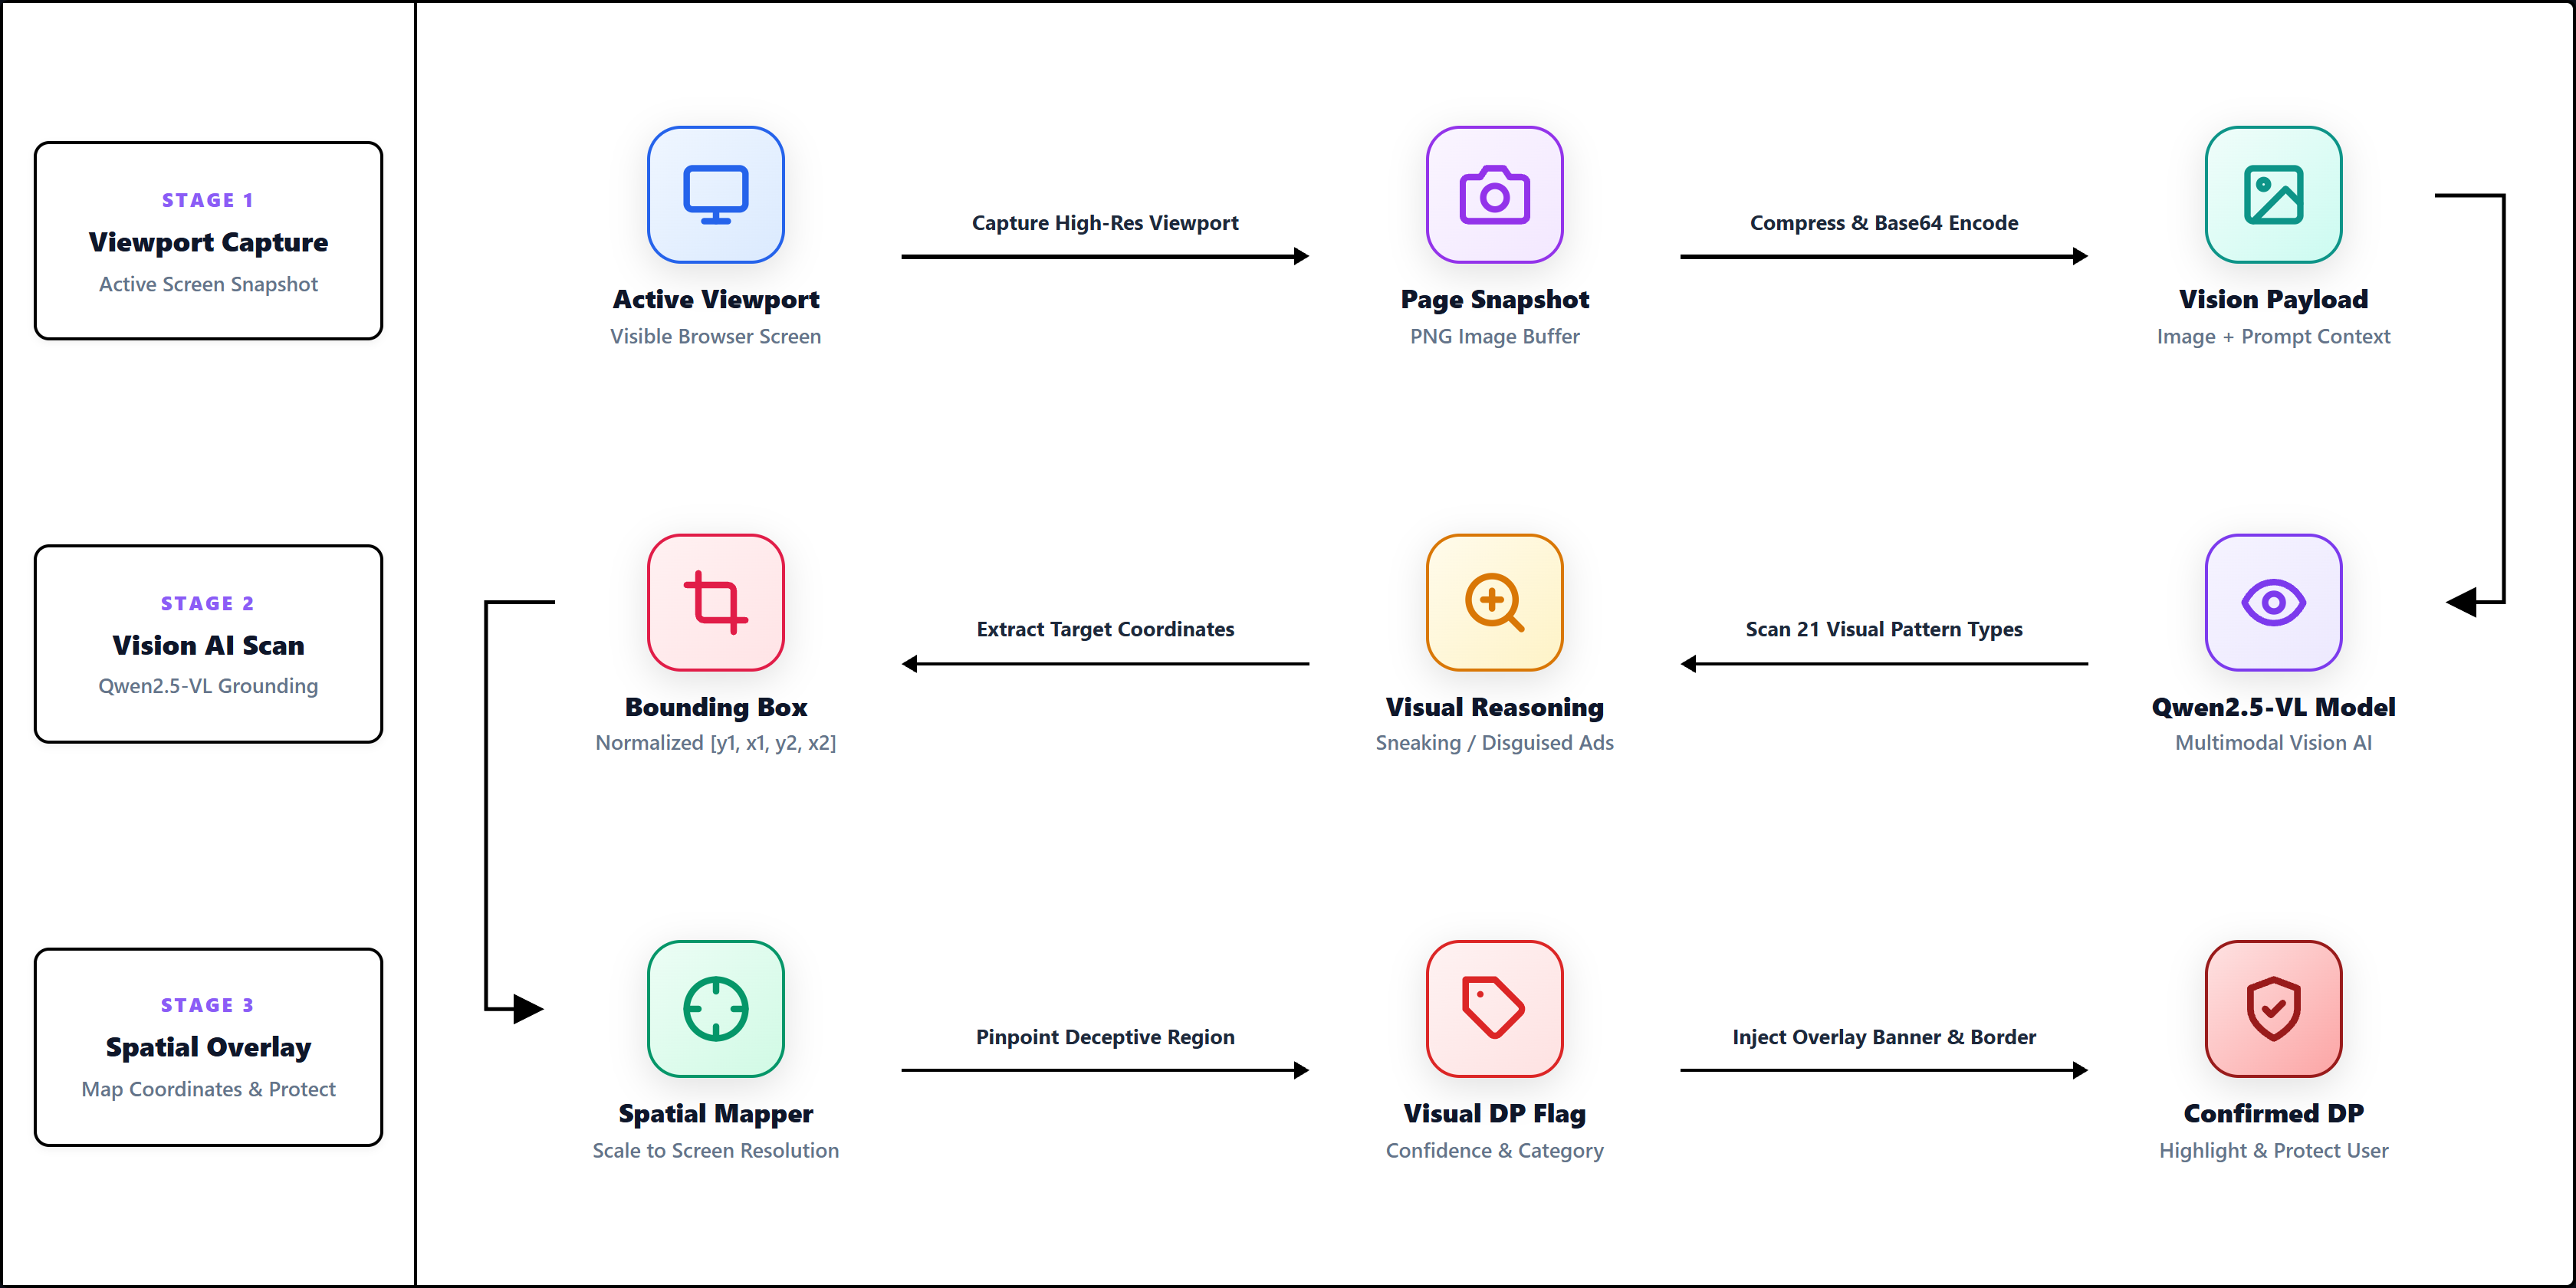
\includegraphics[width=\textwidth]{assets/Visual_Detection_Pipeline_Diagram.png}
    \caption{The Visual Detection Pipeline utilizing Qwen2.5-VL for multimodal spatial reasoning.}
    \label{fig:visual_pipe}
\end{figure}

% --- 6. Countermeasure Pipeline ---
\section{Dynamic Countermeasure Pipeline}
Detection is merely diagnostic; the countermeasure pipeline is therapeutic. An active countermeasure is defined as a direct DOM mutation designed to reduce manipulation and restore user autonomy \cite{schaefer2024}.

\begin{figure}[htbp]
    \centering
    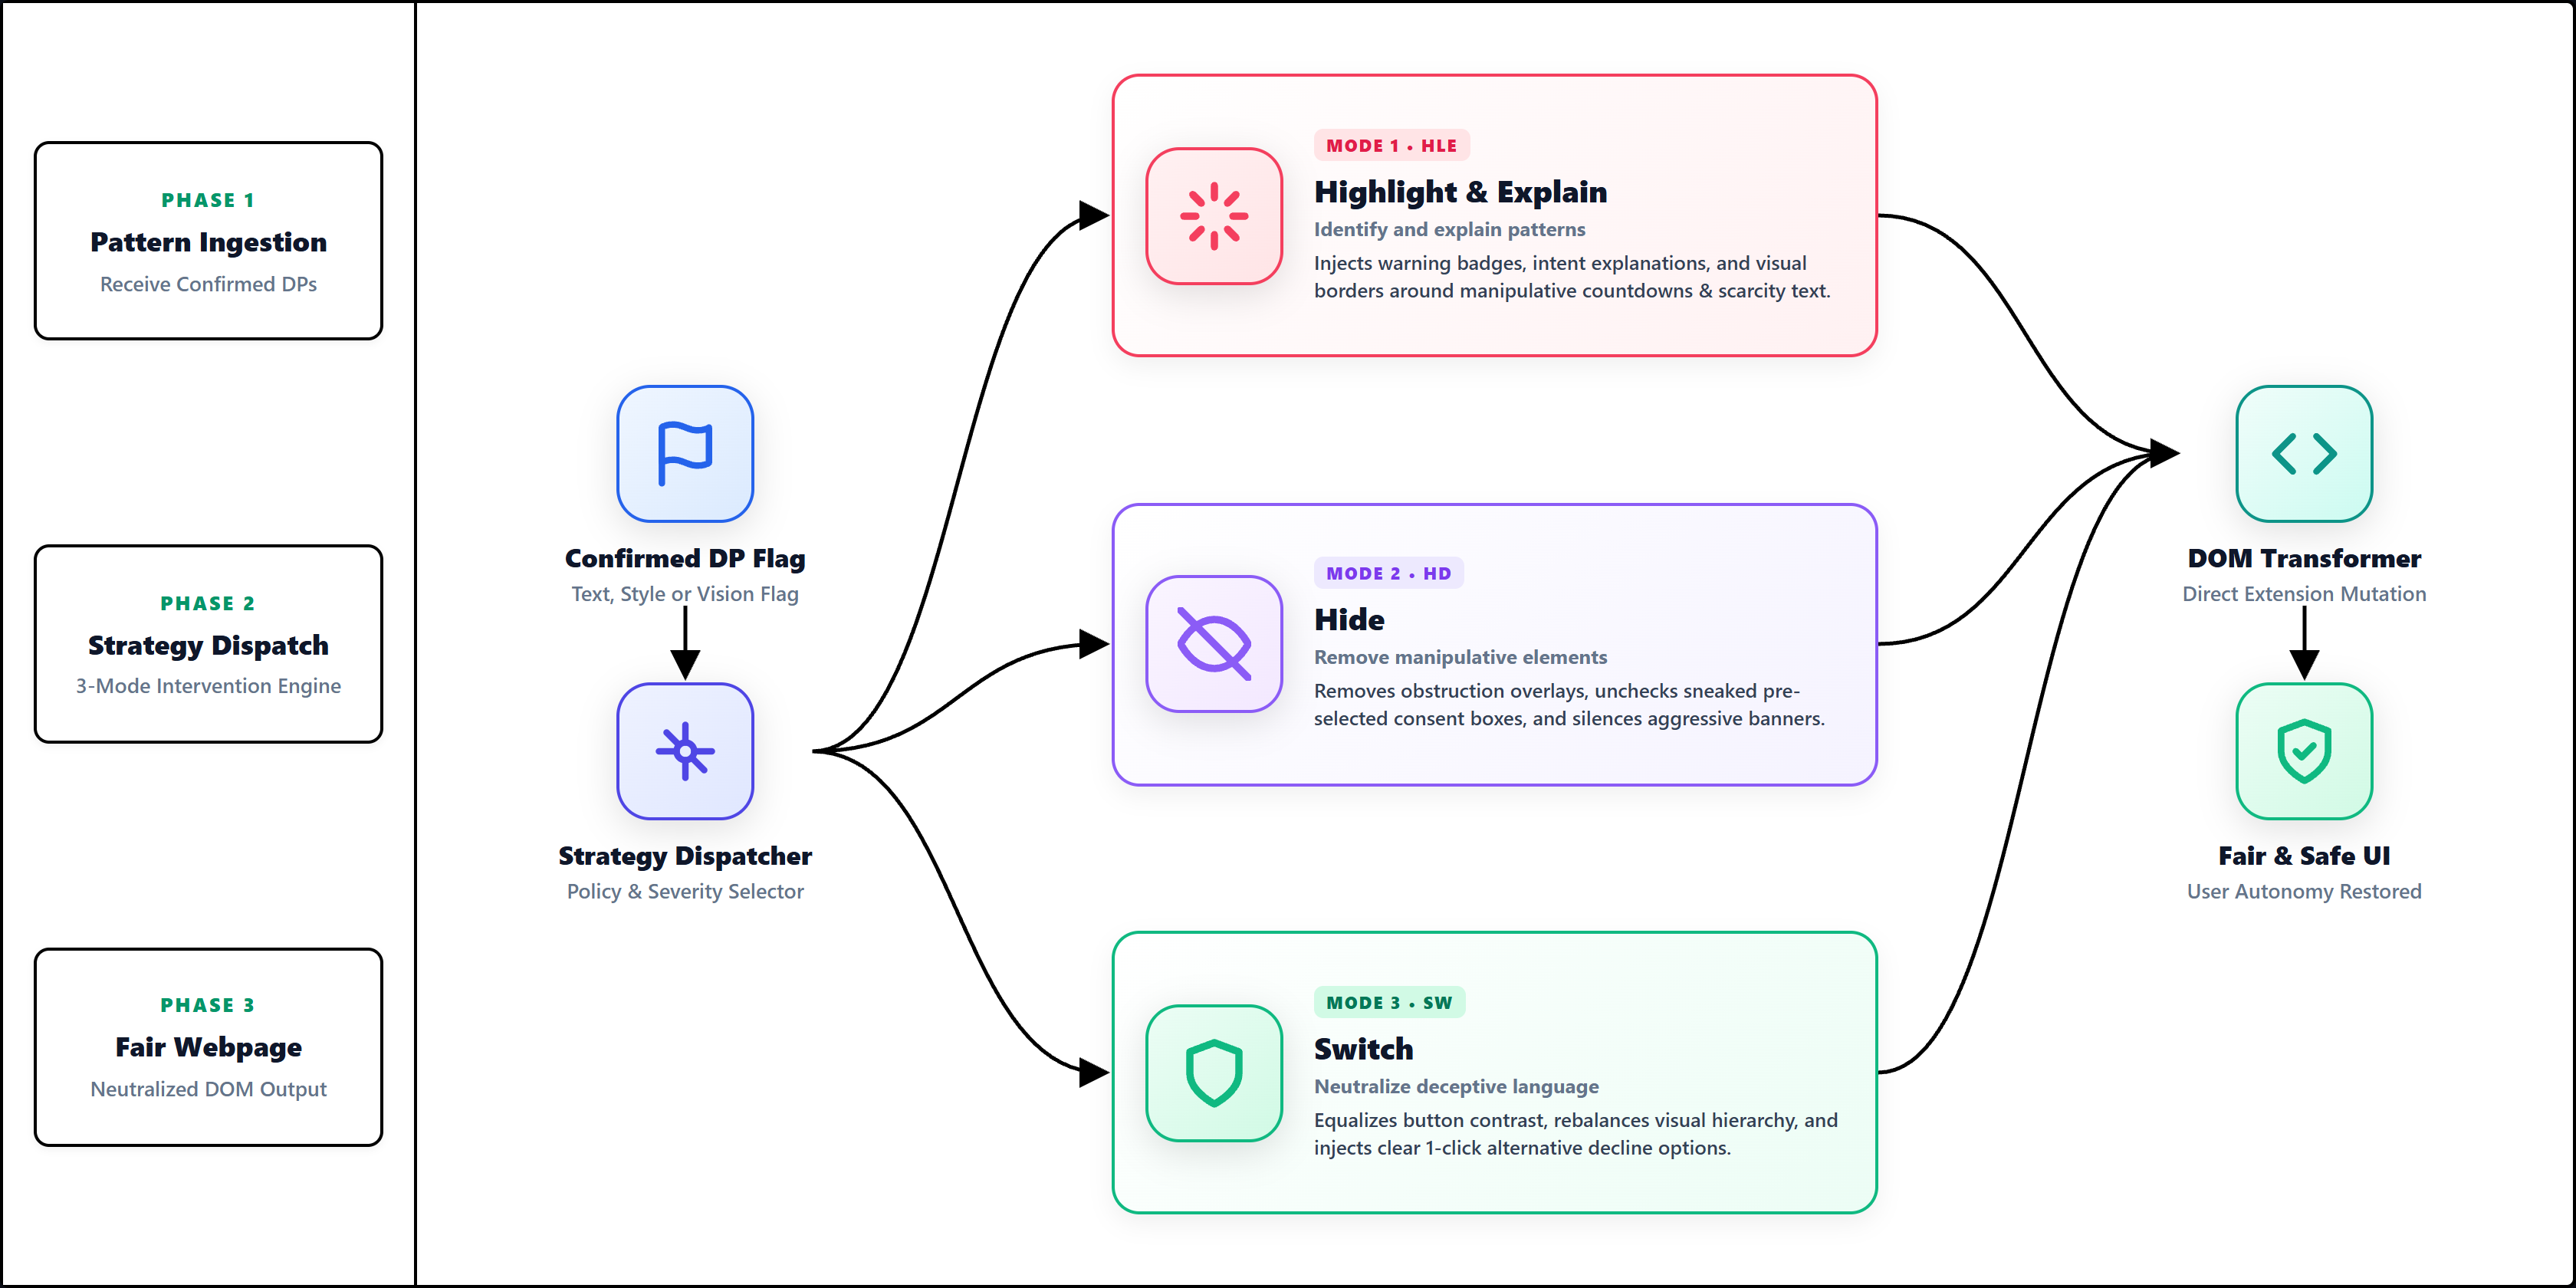
\includegraphics[width=\textwidth]{assets/Countermeasures_Pipeline_Diagram.png}
    \caption{The Countermeasure Pipeline routing detected flags through the user's preferred strategy.}
    \label{fig:countermeasure_pipe}
\end{figure}

\subsection{Strategy Dispatcher and DOM Transformer}
Once any pipeline confirms a dark pattern, the flag is passed to the Strategy Dispatcher. The dispatcher dynamically references the user's active preferences in the extension settings. The dispatcher then signals the DOM Transformer to apply one of three modes \cite{potel, schaefer2024}:

\begin{enumerate}
    \item \textbf{Highlight \& Explain (HLE):} Wraps the manipulative element in a high-visibility, pulsing red border and injects a tooltip explaining the psychological tactic in use.
    \begin{figure}[htbp]
        \centering
        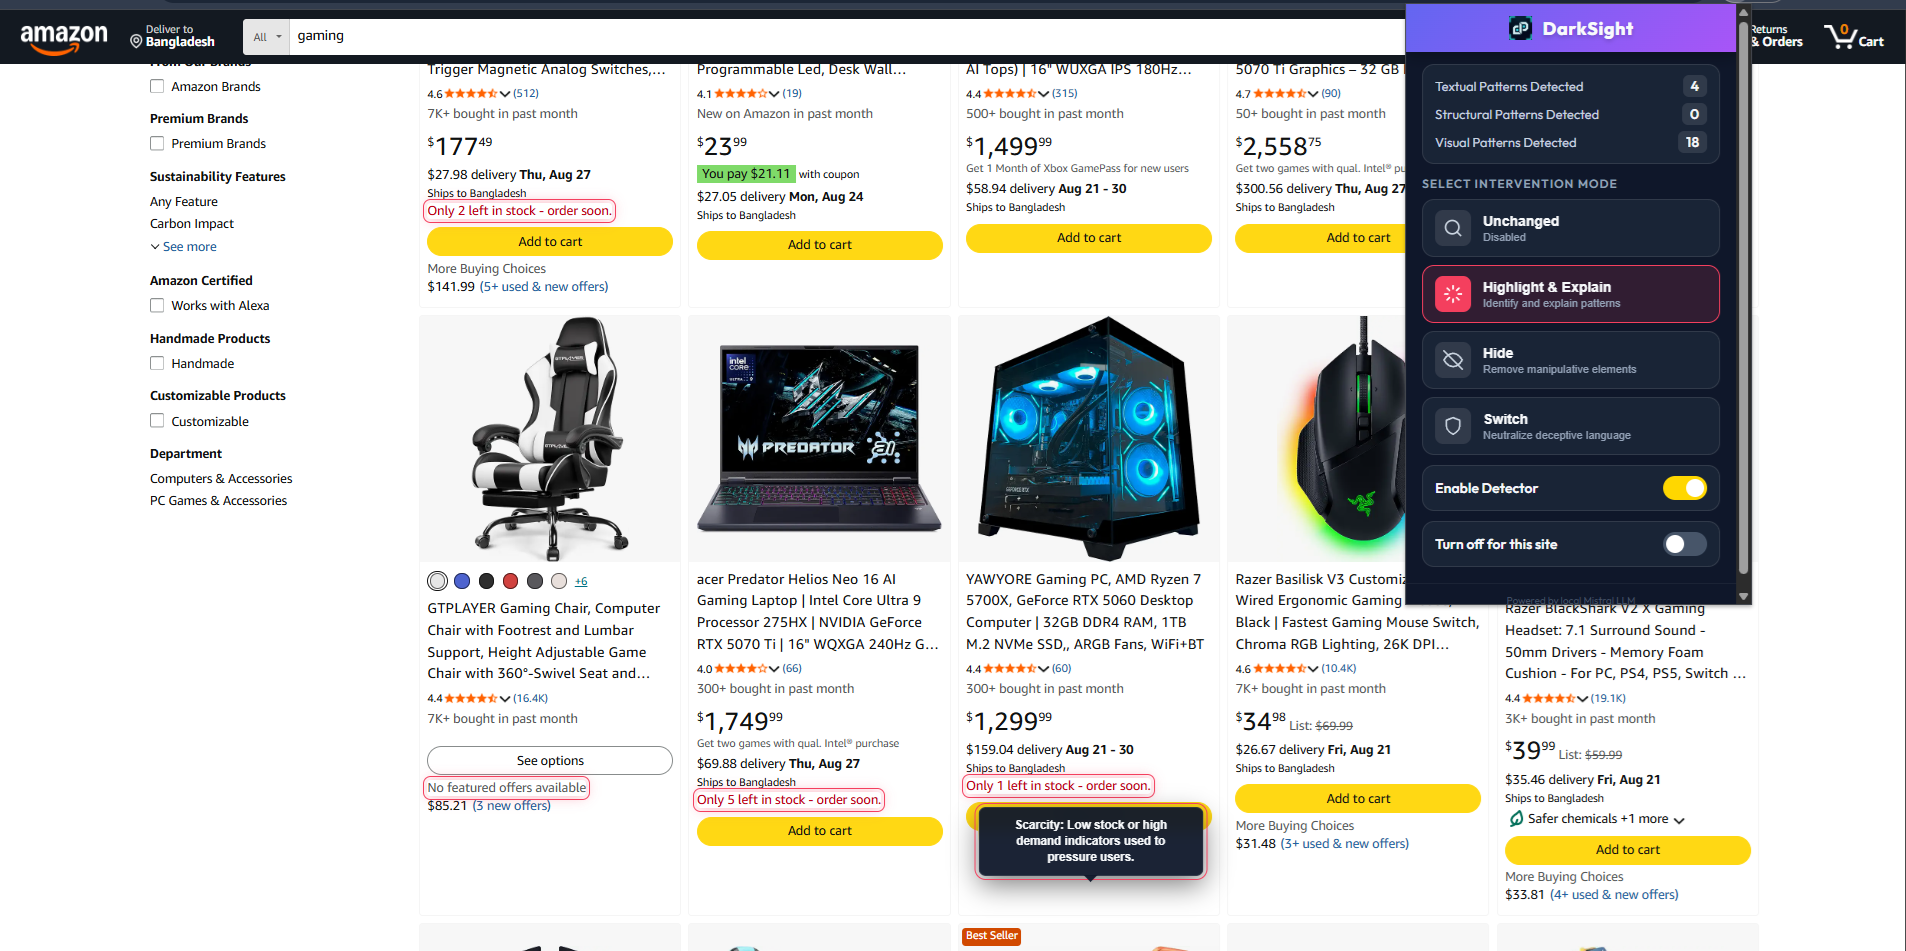
\includegraphics[width=0.8\textwidth]{assets/changes/H_and_E.png}
        \caption{Countermeasure: Highlight \& Explain (HLE) applied to a deceptive element.}
        \label{fig:cm_hle}
    \end{figure}
    
    \item \textbf{Hide (HD):} Completely removes the deceptive element from the DOM (e.g., removing a fake countdown timer) by collapsing its CSS display properties.
    \begin{figure}[htbp]
        \centering
        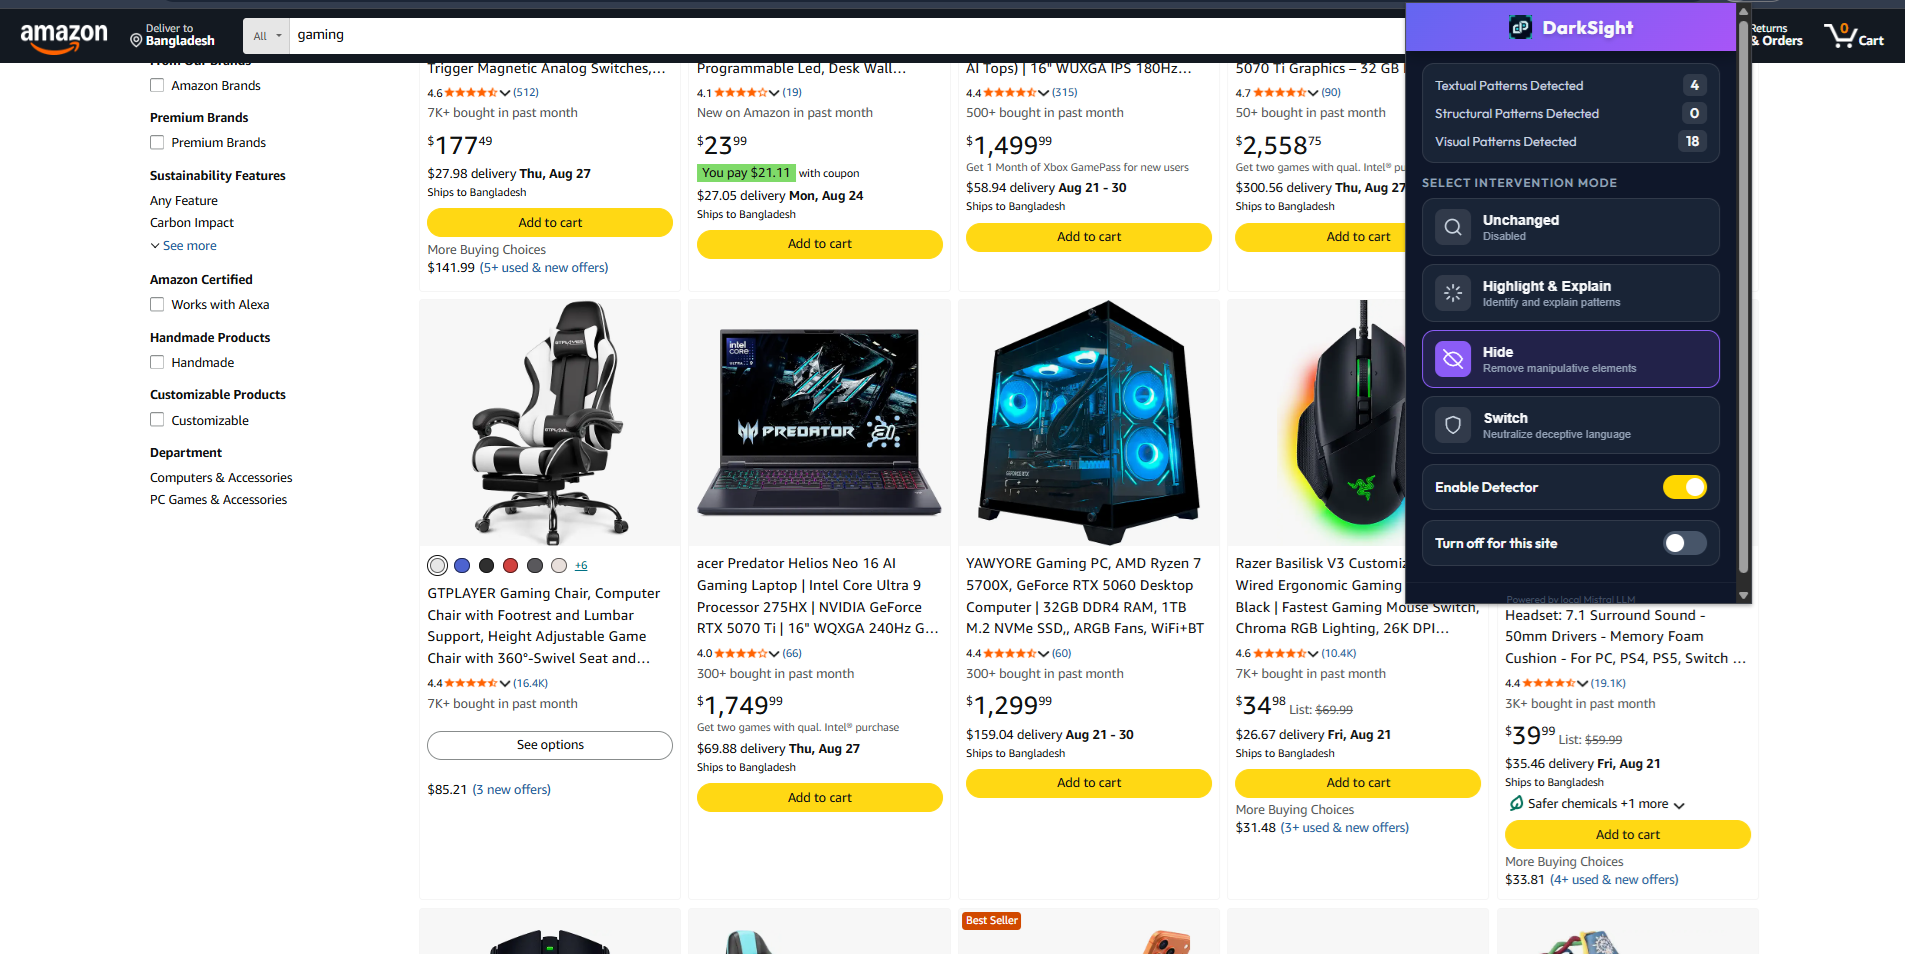
\includegraphics[width=0.8\textwidth]{assets/changes/Hide.png}
        \caption{Countermeasure: Hide (HD) visually suppressing a manipulative component.}
        \label{fig:cm_hide}
    \end{figure}
    
    \item \textbf{Switch (SW):} Neutralizes high-pressure deceptive language by actively replacing the text.
    \begin{figure}[htbp]
        \centering
        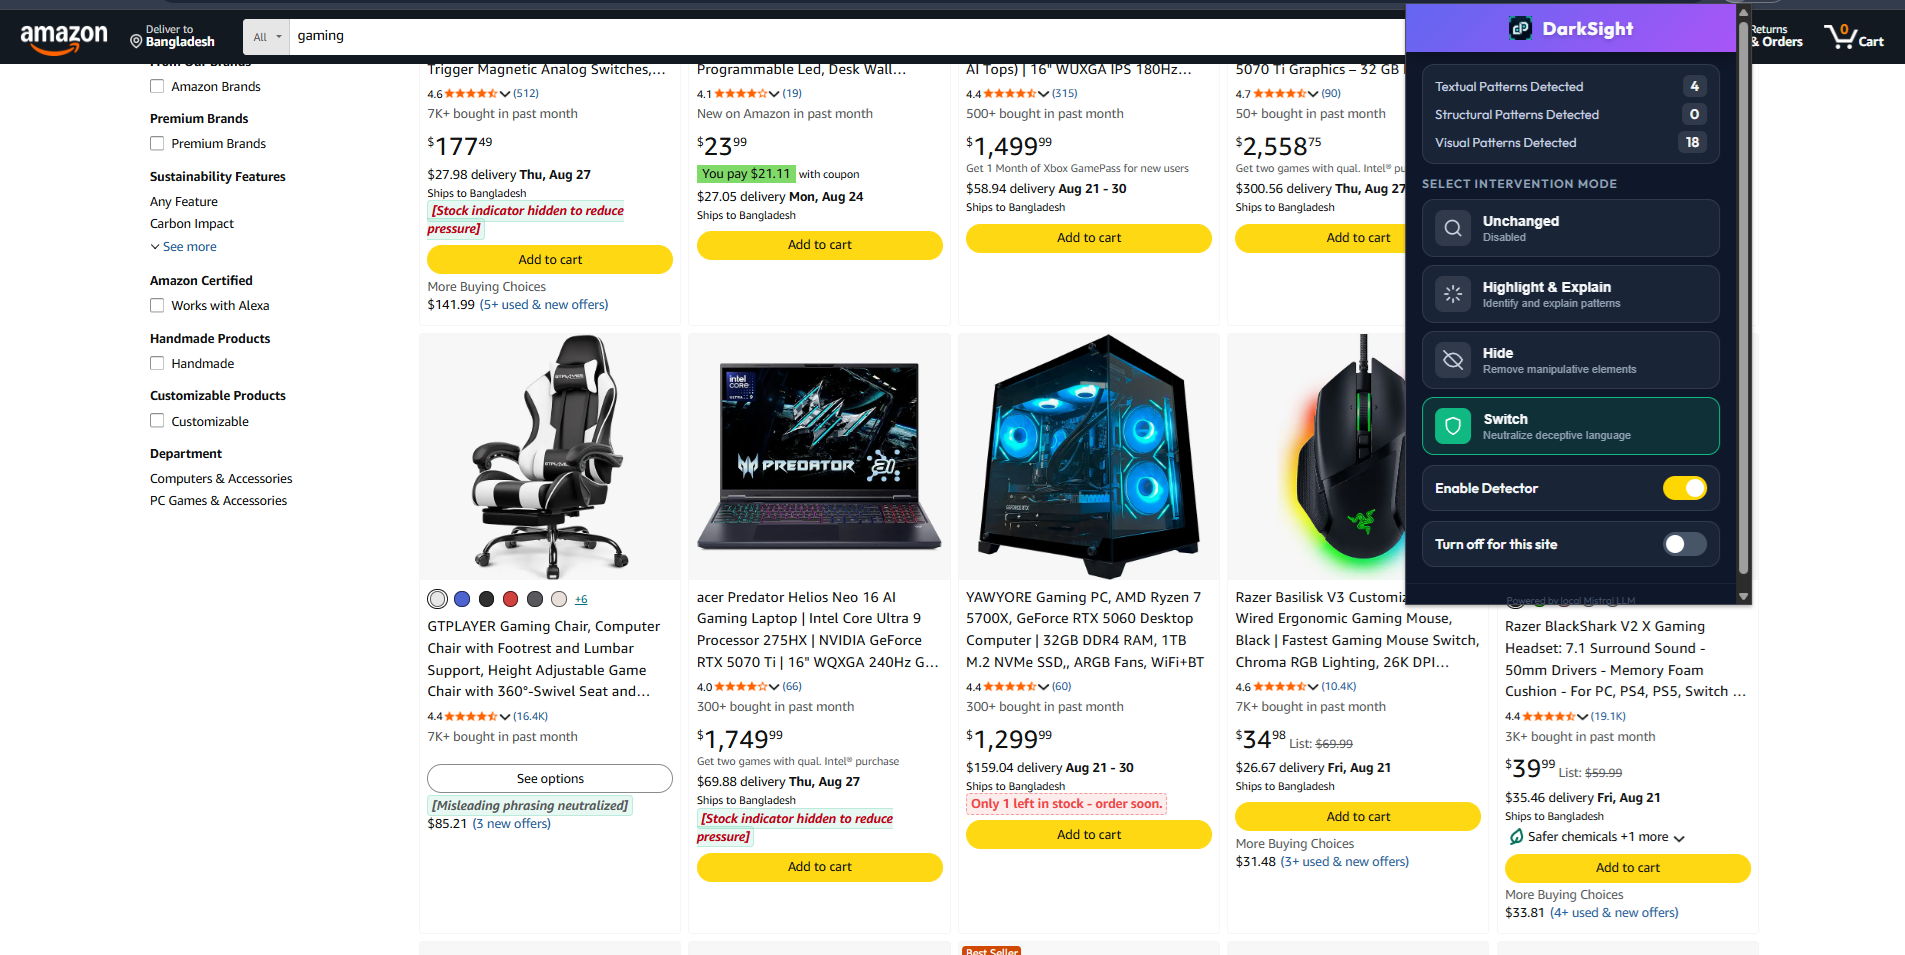
\includegraphics[width=0.8\textwidth]{assets/changes/Switch.png}
        \caption{Countermeasure: Switch (SW) replacing manipulative text with neutral phrasing.}
        \label{fig:cm_switch}
    \end{figure}
\end{enumerate}

% --- 7. Evaluation Setup ---
\section{Evaluation Setup}
To ensure academic rigor, DarkSight was subjected to comprehensive evaluation across three distinct environments. 

\subsection{Dataset Definitions}
\begin{itemize}
    \item \textbf{Textual Evaluation:} We evaluated the regex and LLM (DeepSeek-R1) engines against the Mathur dataset \cite{mathur2019}, comprising 1,818 ground-truth shopping website texts known to harbor dark patterns. 
    \item \textbf{Visual Evaluation:} We evaluated the Qwen2.5-VL pipeline against the AidUI ContextDP image dataset \cite{aidui2023}, consisting of 501 unique images containing 602 deceptive visual instances.
\end{itemize}

\subsection{Real-World E-Commerce Testing}
Beyond static datasets, DarkSight was injected into live production DOMs on major e-commerce platforms. Using a customized headful Puppeteer automation suite, we verified that the DOM Transformer successfully injected real-time countermeasures without breaking site functionality.

% --- 8. Results ---
\section{Results and Discussion}
DarkSight achieved highly robust detection metrics, proving the validity of the hybrid architecture. 

\subsection{Textual Pipeline Accuracy}
The DeepSeek-R1 textual pipeline detected 1,274 patterns out of 1,818 scanned instances, yielding an \textbf{Overall Textual Accuracy of 70.07\%}. The pipeline excels at explicit linguistic patterns like Scarcity (97.35\%) and Social Proof (80.92\%), where high-pressure keywords are abundant. However, text models struggle with visual patterns like Obstruction (19.35\%), which rely heavily on structural UI flows rather than pure text.

\begin{table}[htbp]
\centering
\caption{Results for Dark Pattern Categories (Textual Pipeline)}
\begin{tabular}{|c|l|c|c|c|}
\hline
\textbf{Rank} & \textbf{DP Category} & \textbf{Scanned} & \textbf{Detected} & \textbf{Accuracy (\%)} \\ \hline
1 & Scarcity & 679 & 661 & 97.35\% \\ \hline
2 & Social Proof & 325 & 263 & 80.92\% \\ \hline
3 & Urgency & 481 & 238 & 49.48\% \\ \hline
4 & Misdirection & 270 & 94 & 34.81\% \\ \hline
5 & Sneaking & 26 & 10 & 38.46\% \\ \hline
6 & Obstruction & 31 & 6 & 19.35\% \\ \hline
7 & Forced Action & 6 & 2 & 33.33\% \\ \hline
\end{tabular}
\end{table}

\subsection{Visual Pipeline Accuracy}
The Qwen2.5-VL visual pipeline successfully compensated for the LLM's blind spots, detecting 486 patterns out of 602 scanned visual instances, achieving an \textbf{Overall Visual Accuracy of 80.73\%}. The pipeline achieved a perfect 100\% accuracy on False Hierarchies because it can explicitly "see" the color suppression of decline buttons. Furthermore, its 79.73\% accuracy across 222 instances of Preselection proves its robust scalability against common web traps. 

\begin{table}[H]
\centering
\caption{Results for Dark Pattern Categories (Visual Pipeline)}
\begin{tabular}{|c|l|c|c|c|}
\hline
\textbf{Rank} & \textbf{DP Category} & \textbf{Scanned} & \textbf{Detected} & \textbf{Accuracy (\%)} \\ \hline
1 & Preselection & 222 & 177 & 79.73\% \\ \hline
2 & Nagging & 114 & 102 & 89.47\% \\ \hline
3 & Countdown on Ads & 56 & 43 & 76.79\% \\ \hline
4 & Toying with Emotion & 52 & 40 & 76.92\% \\ \hline
5 & Hidden Information & 38 & 28 & 73.68\% \\ \hline
6 & False Hierarchy & 26 & 26 & 100.00\% \\ \hline
7 & Disguised Ads & 42 & 26 & 61.90\% \\ \hline
8 & Gamification & 22 & 20 & 90.91\% \\ \hline
9 & Social Pyramid & 20 & 14 & 70.00\% \\ \hline
10 & Price Comparison Prevention & 10 & 10 & 100.00\% \\ \hline
\end{tabular}
\end{table}

\subsection{User Evaluation and Impact}
To assess the real-world efficacy and user reception of DarkSight, a cohort of 11 participants evaluated the extension during live browsing sessions. The survey results provided strong validation of the countermeasure approach. 

Participants rated their experience on a 5-point Likert scale across four key metrics. The averages were consistently high across all dimensions:
\begin{itemize}
    \item \textbf{Ease of Use:} 4.0 / 5.0
    \item \textbf{Warning Helpfulness:} 4.27 / 5.0
    \item \textbf{Increased Confidence:} 4.27 / 5.0
    \item \textbf{Overall Satisfaction:} 4.27 / 5.0
\end{itemize}

To illustrate the distribution of responses, Figure \ref{fig:user_eval_chart} details the exact breakdown for the Overall Satisfaction metric.

\definecolor{gfpurple}{HTML}{673AB7}
\begin{figure}[htbp]
    \centering
    \begin{tikzpicture}
        \begin{axis}[
            ybar,
            width=14cm,
            height=6cm,
            ymin=0, ymax=6.5,
            ytick={0,2,4,6},
            xtick={1,2,3,4,5},
            axis y line=none,
            axis x line*=bottom,
            ymajorgrids=true,
            grid style={draw=gray!30},
            bar width=45pt,
            nodes near coords,
            point meta=explicit symbolic,
            every node near coord/.append style={anchor=south, font=\footnotesize, color=black},
            xlabel={Overall Satisfaction Score (1 = Very Dissatisfied, 5 = Very Satisfied)},
            ]
            \addplot[fill=gfpurple, draw=none] coordinates {
                (1,0) [0 (0\%)]
                (2,0) [0 (0\%)]
                (3,1) [1 (9.1\%)]
                (4,6) [6 (54.5\%)]
                (5,4) [4 (36.4\%)]
            };
        \end{axis}
    \end{tikzpicture}
    \caption{Distribution of Overall Satisfaction scores among participants, demonstrating a highly positive consensus.}
    \label{fig:user_eval_chart}
\end{figure}

Beyond numerical satisfaction, the qualitative impact was significant. When asked which countermeasure strategy helped them the most, 91\% of participants (10 out of 11) cited the \textbf{Highlight \& Explain} feature as highly useful, either on its own or in combination with Hide and Switch modes. Furthermore, when asked if they would use DarkSight in their daily browsing, 72.7\% responded "Definitely," 18.2\% responded "Probably," and 9.1\% responded "Maybe." No participants indicated they would decline to use it. 

Regarding future improvements, the majority of users (7 out of 11) requested more extensive customization options within the Countermeasures engine (e.g., customizing colors for different warning levels or adding granular control over the Hide feature). These results confirm that users are highly receptive to active, automated defense against manipulative designs.

% --- 9. Limitations ---
\section{Limitations}
While highly effective, DarkSight currently operates with certain constraints. The multimodal vision model occasionally struggles with perfectly disguised advertisements that seamlessly mimic surrounding editorial content \cite{kocyigit2025}. Countermeasure interventions are currently restricted to three primary visual strategies, which may not cover extremely complex multi-page subscription traps \cite{schaefer2024}. Furthermore, the system relies on English-language interfaces for optimal LLM context parsing.

% --- 10. Future Work ---
\section{Future Work}
Future iterations of DarkSight will focus on improving visual detection accuracy by fine-tuning a proprietary multimodal model specifically on dark pattern UI layouts. We plan to expand the countermeasures engine to support adaptive, personalized protection settings based on individual user demographics and cognitive vulnerabilities, and broaden the architectural framework to support non-English linguistic taxonomies.

% --- 11. Conclusion ---
\section{Conclusion}
DarkSight successfully bridges the critical gap between theoretical academic research and real-world consumer protection. By seamlessly integrating multiple landmark research methodologies into a unified, lightweight, real-time browser extension, we have established a new paradigm in digital defense. Through the DP Sentinel hybrid architecture, DarkSight achieves formidable detection accuracy rates while entirely circumventing the latency constraints of traditional static scanning. Most importantly, by deploying active DOM countermeasures, DarkSight moves beyond mere awareness, actively shielding users and restoring fair, autonomous decision-making to the modern web experience.

% --- References ---
\newpage
\begin{thebibliography}{99}

\bibitem{mathur2019}
A. Mathur, G. Acar, M. J. Friedman, E. Lucherini, J. Mayer, M. Chetty, and A. Narayanan, 
``Dark Patterns at Scale: Findings from a Crawl of 11K Shopping Websites,'' 
\textit{Proceedings of the ACM on Human-Computer Interaction}, vol. 3, no. CSCW, pp. 1--32, 2019.

\bibitem{schaefer2023}
M. Schäfer et al., 
``Taxonomy of Dark Patterns for LLM Analysis,'' 
\textit{2023}.

\bibitem{incontext2023}
``In-Context Learning: Few-Shot Prompt Engineering Methodology,'' \textit{2023}.

\bibitem{dpsentinel2024}
``Dark Pattern Sentinel: A Hybrid DOM Heuristics and LLM-Based Real-Time Detection System,'' \textit{2024}.

\bibitem{50shades}
``50 Shades of Deceptive Patterns: Visual Deception Baseline.''

\bibitem{aidui2023}
``AidUI: Structural Hierarchy Detection,'' \textit{2023}.

\bibitem{schaefer2024}
M. Schäfer, P. Preuschoff, and J. Borchers, 
``Fighting Malicious Designs: Towards Visual Countermeasures Against Dark Patterns,'' 
\textit{Proceedings of the 2024 CHI Conference on Human Factors in Computing Systems}, 2024.

\bibitem{vedha}
R. Vedhapriyavadhana, P. Bharti, and S. Chidambaranathan, 
``Detecting dark patterns in shopping websites – a multi-faceted approach using Bidirectional Encoder Representations From Transformers (BERT).''

\bibitem{bajaj2025}
A. Bajaj, K. Uppal, R. Razdan, Y. Tuteja, A. Bhardwaj, and A. Abraham, 
``A Comprehensive Analysis for Dark Pattern Detection Using Structural, Visual and Textual Information,'' \textit{2025}.

\bibitem{kocyigit2025}
Kocyigit et al., 
``DeceptiLens: An Approach Supporting Transparency in Deceptive Pattern Detection Based on a Multimodal Large Language Model,'' \textit{FAccT 2025}.

\bibitem{cuvin}
P. Cuvin, H. Zhu, and D. Yang, 
``DECEPTICON: How Dark Patterns Manipulate Web Agents,'' \textit{Stanford University}.

\bibitem{luguri}
J. Luguri and L. Strahilevitz, 
``Shining a Light on Dark Patterns.''

\bibitem{chen}
J. Chen et al., 
``Unveiling the Tricks: Automated Detection of Dark Patterns in Mobile Applications.''

\bibitem{potel}
M. Potel-Saville and M. Da Rocha, 
``From Dark Patterns to Fair Patterns? Usable Taxonomy to Contribute Solving the Issue with Countermeasures.''

\bibitem{raju}
Dr. S. Hrushikesava Raju,
``Smart dark pattern detection: Making aware of misleading patterns through the intended app.''

\bibitem{yada_ui}
Y. Yada,
``Why is the User Interface a Dark Pattern? :Explainable Auto-Detection and its Analysis,'' Dec 2023.

\bibitem{nie}
M. Nie,
``Algorithmic Addiction by Design: Big Tech’s Leverage of Dark Patterns to Maintain Market Dominance and its Challenge for Content Moderation.''

\bibitem{darkarts}
``Defending Against the Dark Arts: Recognising Dark Patterns in Social Media.''

\bibitem{mathur_what}
A. Mathur, J. Mayer, and M. Kshirsagar,
``What Makes a Dark Pattern... Dark? Design Attributes, Normative Considerations, and Measurement Methods,'' Princeton University.

\bibitem{karagoel}
I. Karagoel and D. Nathan-Roberts,
``Dark Patterns: Social Media, Gaming, and E-Commerce.''

\bibitem{hausner}
P. Hausner and M. Gertz,
``Dark Patterns in the Interaction with Cookie Banners.''

\bibitem{sin}
R. Sin, T. Harris, S. Nilsson, and T. Beck,
``Dark patterns in online shopping: do they work and can nudges help mitigate impulse buying?''

\bibitem{uiguard}
``UIGuard: Automated Detection of Dark Patterns in Mobile Applications,'' \textit{UIST 2023}.

\bibitem{schaefer_investigating}
R. Schäfer, P. Preuschoff, and J. Borchers,
``Investigating Visual Countermeasures Against Dark Patterns in User Interfaces.''

\bibitem{li}
M. Li et al.,
``A Comprehensive Study on Dark Patterns,'' \textit{Shenzhen Technology University, China}.

\bibitem{yada_dataset}
Y. Yada et al.,
``Dark patterns in e-commerce: a dataset and its baseline evaluations.''

\end{thebibliography}

\end{document}
